
 \documentclass[a4paper,12pt,oneside]{book}
 %\documentclass[a4paper,12pt]{report}
\usepackage[italian]{babel}
\usepackage[latin1]{inputenc}
\usepackage{amsfonts}
\usepackage{amsmath}
\DeclareMathOperator*{\argmin}{argmin}
\usepackage{empheq}
\usepackage{bmpsize}
\usepackage{hyperref}
\usepackage{breakurl}
\setcounter{tocdepth}{2}
\usepackage[dvipdfm]{graphicx}
\usepackage{graphicx}
\usepackage[formats]{listings}
\linespread{1.5}
\begin{document}
\lstset{language=Python, showspaces=false, showstringspaces=false}
\thispagestyle{empty}
\begin{figure}
\centering

\includegraphics[scale=0.30]{Logo}
\end{figure}
\begin{center}
\textbf{UNIVERSIT\`{A} DEGLI STUDI "ROMA TRE"}\\
%\vspace{0.18cm}
\textmd{\large Dipartimento di Matematica e Fisica}\\
%\vspace{0.18cm}
\large{ Corso di Laurea Magistrale in Scienze Computazionali}\\	
%\vspace{1.35cm}	
\textmd{\Large{Tesi di Laurea Magistrale}}\\
\vspace{1cm}
\LARGE{\LARGE{\textbf{Ricerca della topologia ottimale di un sistema di deep learning per identificazioni di oggetti architettonici}}}\\
\vspace{3.5cm}
\begin{tabular}{ccccccccccc}
	\large{\textbf{Candidato}}& & & & & & & & & & \large{\textbf{Relatore}}\\
	\large{D\'{e}sir\'{e}e Adiutori} & & & & & & & & & &\large{Prof. Luciano Teresi}\\
	& & & & & & & & & & \large{\textbf{Correlatore}}\\
	& & & & & & & & & & \large{Prof. Roberto D'Autilia}
\end{tabular}\\
\vspace{1.4cm}
\normalsize{Anno Accademico 2017/2018}
\end{center}
\newpage

\tableofcontents

\newpage
\section*{Introduzione}
\addcontentsline{toc}{section}{Introduzione}
Dall'invenzione dei computer, l'uomo fa sempre pi\`{u} affidamento sulle macchine per risolvere problemi complessi di calcolo. Con l'aumentare delle prestazioni dei computer, man mano si sono sviluppati algoritmi di calcolo sempre pi\`{u} efficienti.
Nel 1959 l'ingegnere del MIT, Arthur Samuel coni\`{o} il termine \textit{"machine learning"}, descrivendo l'apprendimento automatico come un "campo di studio che d\`{a} ai computer la possibilit\`{a} di apprendere senza essere programmati esplicitamente per farlo".\cite{Samuel} \\
Definiamo l'apprendimento automatico come un insieme di metodi in grado di rilevare automaticamente i modelli tramite dei dati e quindi utilizzare i modelli scoperti per prevedere i dati futuri o per eseguire altri tipi di processi decisionali in condizioni di incertezza. L'insegnamento alla macchina \`e, pertanto, imprescindibile dai dati. Generalmente, pi\`{u} dati si passano alla macchina, pi\`{u} pu\`{o} imparare. Per questo motivo, con l'avvento di Internet, dagli anni '90 ad oggi, il tema del "machine learning" \`e diventato sempre pi\`{u} attuale. La mole di dati reperibile dal web \`e cospicua ed ha permesso che questo campo sia esponenzialmente progredito.\\
Il \textit{"deep learning"} \`e un tipo particolare di machine learning, che riguarda l'emulazione di come gli esseri umani apprendono. Esso affronta i problemi del machine learning, rappresentando il mondo come una gerarchia di concetti annidati: ogni concetto \`e definito in relazione a concetti pi\`{u} semplici e le rappresentazioni astratte vengono calcolate in termini di concetti meno astratti. Il Deep Learning implica l'utilizzo di reti neurali artificiali (\textit{deep artificial neural networks}) algoritmi e sistemi computazionali, ispirati al cervello umano, per affrontare i problemi del Machine Learning.\\
L'analogia di Shehzad Noor Taus Priyo pu\`{o} aiutare a capire meglio cosa siano le reti neurali:\\
"Immaginiamole come una serie di porte da passare, dove l'input \`e l'uomo che le deve oltrepassare e ogni volta che lo fa cambia qualcosa nel suo comportamento finch\'{e}, all'ultima porta oltrepassata, l'uomo \`e diventato una persona del tutto differente, rappresentando l'output di questo processo."\cite{analogia} \\
Questa tesi si focalizza su un problema particolare di machine learning: la Classificazione (\textit{Classification}) in particolar modo di immagini. L'obiettivo principale \`e trovare un'architettura ottimale per l'algoritmo che identifica le immagini di oggetti architettonici, inserendo tra i parametri anche le coordinate geofisiche dell'oggetto. Per fare questo bisogna trovare la giusta topologia, la giusta profondit\`{a} e la giusta larghezza di ogni livello della rete neurale, in due parole: l'architettura ottimale.\\
Nel primo capitolo si descrive cosa sono e come sono strutturati gli algoritmi di apprendimento. Nel secondo si introduce il concetto di rete neurale, ponendo particolare attenzione sulle reti neurali di tipo convoluzionale. Nel terzo si descrive il linguaggio di programmazione TensorFlow di Python, mostrando alcuni esempi concreti di programmazione per la classificazione di oggetti; in particolar modo viene mostrato il codice utilizzato per la classificazione di oggetti architettonici e quello per la realizzazione di un App, per dispositivo Android, che lo implementi (prevalentemente codice Java). Infine nell'ultima parte vengono mostrati i risultati ottenuti.
 
\chapter{Algoritmi di apprendimento}
Gli algoritmi di machine learning sono solitamente divisi in tre tipi principali:
\begin{itemize}
\item Supervised learning (apprendimento supervisionato)
\item Unsupervised learning (apprendimento non supervisionato)
\item Reinforcement learning (apprendimento per rinforzo)
\end{itemize}
Quali usare? Perch\'{e} sceglierne uno piuttosto che un altro?\\
La scelta dell'algoritmo da utilizzare dipende dal tipo di dati di cui si dispone. Ma la scelta finale va fatta solo esclusivamente dopo aver testato l'algoritmo, e si sceglie in base a quello pi\`{u} performante: un insieme di ipotesi che funziona bene in un dominio, potrebbe funzionare male in un altro.\\
\textbf{Teorema del No Free Lunch \cite[Wolper,1996]{NFL}}\\
\textit{Non esiste una definizione universale di algoritmo "migliore".}
\section{Costruzione di un algoritmo}\label{Costruzione}
Per costruire un algoritmo di apprendimento bisogna avere:
\begin{itemize}
\item processi(\textit{task}): compiti che l'algoritmo deve eseguire;
\item misuratori di rendiment: rilevatori delle caratteristiche dei processi;
\item esperienze: quantit\'{a} di dati dal quale imparare.
\end{itemize}
I processi di apprendimento automatico descrivono come il sistema dovrebbe elaborare un esempio.
\newtheorem{defin}{Definizione}
\begin{defin}
Un \textbf{esempio} \`e una raccolta di caratteristiche che sono state misurate quantitativamente da alcuni oggetti o eventi elaborati. 
\end{defin}
Di solito, un esempio viene rappresentato da un vettore $x\in \mathbb{R}^{n}$, dove ogni elemento $x_{i}$ rappresenta una caratteristica.\\
Ad esempio, se si considera un fiore: le caratteristiche che lo descrivono sono la lunghezza e la larghezza dei suoi petali e il colore. Quindi in questo caso la metrica usata \`e la distanza euclidea tra le due estremit\`{a} del petalo:\\
se si considera $x=(x_1,x_2,x_3)$ il fiore con queste 3 caratteristiche, si ha che:
$$x_{1}=d(h_{min},h_{max})\qquad x_{2}=d(b_{min},b_{max})\qquad x_{3}=stringa$$
dove $h_{min}$ e $h_{max}$ rappresentano i due punti relativi alle estremit\`{a} del petalo e $d:\mathbb{R} \times \mathbb{R} \longrightarrow \mathbb{R}$    t.c   $d(x,y)=\sqrt{(x-y)^{2}}=|x-y|$.\\
Dato un processo si cerca di capire quale sia la caratteristica principale, sulla quale si deve misurare il suo rendimento.
Infine, dobbiamo dare all'algoritmo un'esperienza sulla quale apprendere, che \`e quella che lo classificher\`{a} in uno dei tre tipi principali.
Questa esperienza l'apprende dai \textit{dataset}: una collezione di esempi.\\
I dataset possono essere di vari tipi:
\begin{itemize}
\item di addestramento ( \textit{training set})
\item di prova ( \textit{test set})
\item di validazione ( \textit{validation set})
\end{itemize}
L' \textbf{insieme di addestramento} \`e una parte dell'insieme di dati che vengono utilizzati per addestrare un sistema di apprendimento supervisionato.\\
Da questo insieme, l'algoritmo deve costruire una funzione che capisca, dai parametri, quali caratteristiche descrivono le varie categorie.\\
L' \textbf{insieme di prova} \`e un insieme di dati che, con l'insieme di addestramento, forma una partizione del dataset di partenza. Questi nuovi dati vengono utilizzati per valutare l'apprendimento dell'algoritmo "addestrato".\\
L' \textbf{insieme di validazione} \`e usato in maniera analoga all'insieme di prova, ma dei dati inseriti per testare l'algoritmo gi\`{a} si conosce la risposta (una parte di essi pu\`{o} far parte dell'insieme di addestramento) e da questa si valuta se l'output ottenuto \`e ottimale o meno.\\
Questi tre insiemi possono coesistere e la scelta delle loro cardinalit\`{a} non \`e universale: dipende dal tipo di problema che viene affrontato.\\
Vediamo ora come valutare l'efficienza di un algoritmo:
\begin{defin}
L'\textbf{errore di allenamento}(\textit{training error}) \`e una misura di errore che si pu\`{o} calcolare sul set di allenamento. Indica quanto l'algortimo sta apprendendo.
\end{defin}
\begin{defin}
La \textbf{generalizzazione} \`e la capacit\`{a} di un algoritmo di essere ottimale in seguito ad un input proveniente dall' insieme di prova.
\end{defin}
\begin{defin}
L'\textbf{errore di generalizzazione}(\textit{generalization error}) \`e una misura di errore che si pu\`{o} calcolare sull'insieme di prova. Verifica se l'algoritmo ha imparato o solo memorizzato.
Esso viene detto anche errore di test (\textit{test error}).
\end{defin}
Si ipotizza che tutti gli esempi siano eventi indipendenti e che tuti gli insiemi, in cui si partiziona l'insieme di dati, hanno la stessa distribuzione di probabilit\`{a} uniforme.
\begin{defin}
Una \textbf{funzione di perdita} (\textit{loss function}) $$L(y,\hat{y}):\mathbb{R}^{n} \times \mathbb{R}^{n} \rightarrow \mathbb{R}$$ \`e una funzione che misura la distanza (o l'errore) tra i valori di output previsto $\hat{y}$ e i valori effettivi ${y}$.
\end{defin}
Si possono usare varie misure, ad esempio l'errore quadratico medio(MSE):
\begin{equation}\label{train-error}
L(y,\hat{y})_{train}=\frac{1}{n}\sum_{i=1}^{n}(\hat{y}_{(train)}-y_{(train)})_{i}^2
\end{equation}
La funzione di predizione dipender\`{a} da dei parametri, rappresentati da un vettore $w$, lo scopo \`e di minimizzare l'errore di allenamento variando $w$.
In base al tipo di apprendimento e al problema da affrontare, verranno usati vari algoritmi per risolvere problemi di minimizzazione libera. Gli algoritmi che risolverono il problema:
\begin{equation}\label{minimi}
f(x^{*})=\min_{x\in \mathbb{R}^{n}}f(x),\qquad \qquad f\in C^{2}(\mathbb{R}^{n},\mathbb{R})
\end{equation}
Per risolvere problemi di questo tipo, spesso viene utilizzato il metodo di discesa del gradiente \cite{an}. \\
La struttura generale di un metodo di discesa iterativo di minimizzazione \`e:
\begin{equation}\label{eq:min}
x_{k+1}=x_{k}+\beta_{k}d_{k}
\end{equation}
dove $x_k$ rappresenta il valore della x al k-esimo passo. Si parte dal valore $x_{0}$ assegnato, $\beta_{k}\in \mathbb{R^{+}}$ \`e il passo e $d_{k}\in \mathbb{R}^{n}$ \`e la direzione lungo la quale ci si muove che, essendo di discesa, sar\`{a} tale che: $(d_{k},\nabla f(x_{k}))<0$. Sia il passo che la direzione vanno scelti opportunamente ad ogni iterazione, in modo che $$f(x_{k+1})<f(x_{k})$$
Per ogni passo imponiamo:
$$f(x_{k}+\beta_{k}d_{k})=\min_{\beta}\{f(x_{k}+\beta d_{k})\}\qquad \qquad (strategia\: \: di\: \: ricerca\: \: esatta)$$
Mentre per la direzione: $d_{k}=-\nabla f(x_{k})$. La derivata direzionale di $f$ nella direzione $d_{k}$ vale $$\frac{\partial f}{\partial d_{k}}(x_{k})=\frac{(d_{k},\nabla f(x_{k}))}{\parallel d_{k}\parallel}=-\parallel \nabla f(x_{k})\parallel$$ e per la disuguaglianza di Cauchy-Schwartz si ha anche: $$\frac{\mid (d_{k},\nabla f(x_{k}))\mid}{\parallel d_{k}\parallel}\leq \frac{\parallel d_{k} \parallel \parallel \nabla f(x_{k})\parallel}{\parallel d_{k}\parallel}=\parallel \nabla f(x_{k})\parallel$$ che mostra come la direzione di ricerca sia quella in cui la derivata direzionale di $f$ \`e negativa e di modulo massimo.\\
Le condizioni di arresto del metodo sono: 
$$\parallel x_{k+1}-x{k}\parallel \leq m,\qquad \parallel \nabla f(x_{k+1})\parallel \leq m\prime$$ oppure: $$k>k_{max}$$ dove $m$ e $m'$ sono soglie date e $k_{max}$ il numero massimo di iterazioni da effettuare.\\
I risultati ottenuti sono garantiti dai seguenti teoremi di convergenza:
\newtheorem{teo}{Teorema}
\begin{teo}
Sia $f(x)\in C^{1}$, strettamente convessa sull'insieme\\ $\Sigma_{0}=\{x\in\mathbb{R}^{n}:f(x)\leq f(x_{0})\}$, e la successione $\{x_{k}\}$ sia generata tramite l'algoritmo (\ref{eq:min}). Si supponga:
\begin{enumerate}
\item che l'insieme $\Sigma_{0}$ sia compatto;
\item che le direzioni $d_{k}$ siano t.c. $\frac{(d_{k},\nabla f(x_{k}))}{\parallel d_{k} \parallel \parallel \nabla f(x_{k})\parallel}\leq - \cos \theta$ per $k\in \textit{I}$, con $\textit{I}$ insieme illimitato di indici;
\item che per $k\in \textit{I}$, $\beta_{k}$ sia ottenuto tramite ricerca esatta.
\end{enumerate}
Allora la successione $\{x_{k}\}$ converge all'unico punto $x^{*}$ di minimo per $f$.
\end{teo}
\begin{teo}
Sia $f(x)\in C^{2}$, strettamente convessa sull'insieme (che si suppone compatto) $\Sigma_{0}=\{x\in\mathbb{R}^{n}:f(x)\leq f(x_{0})\}$, e la successione $\{x_{k}\}$ sia generata tramite l'algoritmo (\ref{eq:min}) con $d_{k}=-\nabla f(x_{k})$.\\
Allora, se i passi $\beta_{k}$ sono determinati tramite ricerca esatta, la successione $x_{k}$ converge all'unico punto $x^{*}$ di minimo per f.
\end{teo}
Minimizzare l'errore di allenamento non necessariamente comporta l'ottimizzazione di apprendimento dell'algoritmo, potrebbe verificarsi il fenomeno di adattamento insufficiente (\textit{underfitting}) ovvero non si hanno abbastanza dati per creare un modello di predizione accurato. Bisogna quindi valutare anche altri fattori: analizzare l'insieme di prova.\\
Ricordandoci dell'eq.\ref{train-error} calcoliamo l'errore di prova:
\begin{equation}\label{test-error}
L(y,\hat{y})_{test}=\frac{1}{n}\sum_{i=1}^{n}(\hat{y}_{(test)}-y_{(test)})_{i}^2
\end{equation}
Vorremmo che, con i parametri trovati per minimizzare l'errore di allenamento, anche questo errore sia minimo (l'ottimalit\`{a} \`e 0). Ma come detto in precedenza non sempre questo accade, vorremmo quindi che il divario tra i due errori sia minimo. In caso contrario si verifica il fenomeno di adattamento eccessivo (\textit{overfitting}) del modello all'insieme di dati che descrive, tramite un eccessivo numero di parametri. Il modello quindi non sar\`{a} generalizzabile ad un nuovo insieme di dati.\\
Consideriamo il valore atteso dell'errore di prova, calcolato prendendo una coppia di punti $(X,Y)$ dall'insieme di prova:
\begin{equation}\label{test}
\mathbb{E} [L(y,\hat{y})_{test}]=\mathbb{E} [(Y-\hat{y}(X))^{2}]
\end{equation}
e definiamo la funzione dell'output effettivo come:
$$y(X)=\mathbb{E}(Y|X)$$
la quale avr\`{a} sicuramente un errore, dovuto da qualche interferenza,\\
che chiameremo: distorsione stimata (\textit{estimation bias}).\\
Ma con diversi insiemi di allenamento, possiamo costruire diverse funzioni $\hat{y}$, e anche questo \`e un'altra fonte di errore: la varianza stimata (\textit{estimation variance}). Possiamo quindi scrivere l'output come:
$$Y=y(X)+\epsilon$$ con $\epsilon$ variabile aleatoria indipendente da $X$ , con $X$ distibuzione normale tale che: $\mathbb{E}[X]=0$ e $Var(X)=\sigma^{2}$.\\
Possiamo quindi riscrivere l'equazione \ref{test} come:
\begin{eqnarray}
\mathbb{E} [L(y,\hat{y})_{test}] &=&\mathbb{E} [(Y-\hat{y}(X))^{2}|X=x]\nonumber\\
&=&\mathbb{E}[(Y-y(x))^2 |X=x]+\mathbb{E}[(y(x)-\hat{y}(x))^{2}|X=x]\nonumber\\
&=&\sigma^{2}+\mathbb{E}[(y(x)-\hat{y}(x))^{2}]
\end{eqnarray}
dove $\sigma^{2}$ \`e chiamato errore Bayes e
\begin{eqnarray}
\mathbb{E}[(y(x)-\hat{y}(x))^{2}]&=&(\mathbb{E}[\hat{y}(x)]-y(x))^{2}+\mathbb{E}[(\hat{y}(x)-\mathbb{E}[\hat{y}(x)])^{2}]\nonumber\\
&=&Bias(\hat{y}(x))^{2}+Var(\hat{y}(x))
\end{eqnarray}
Si ottiene cos\'{\i} il compromesso distorsione-varianza (\textit{bias-variance tradeoff}):
\begin{equation}
\mathbb{E} [L(y,\hat{y})_{test}]=\sigma^2+Bias(\hat{y}(x))^2 + Var(\hat{y}(x))
\end{equation}
Se la distorsione ha valori alti e la varianza bassi avremo un fenomeno di adattamento insufficiente, mentre se la distorsione ha valori bassi e la varianza alti avremo un adatteamento eccessivo.\cite{errval}\\
Un modo per equilibrare questo compromesso \`e usare la convalida incrociata (\textit{Cross-Validation}), che consiste nel ripetere l'addestramento e il test dell'algoritmo ogni volta su sottoinsiemi scelti in maniera casuale.
\section{Apprendimento supervisionato}
Gli algoritmi di apprendimento supervisionato vengono utilizzati per risolvere problemi di classificazione e di regressione, che analizzeremo rispettivamente nel cap. \ref{classificazione} e nel paragrafo \ref{regressione}.\\
Si parla di apprendimento supervisionato quando il dataset che si utilizza contiene delle variabili, una delle quali \`e un'etichetta.\\
Dato un vettore di input $x=(x_{1},\cdots,x_{n})$ ogni $x_{i}$ \`e un vettore d-dimensionale di numeri rappresentanti una caratteristica, da questi dati si costruisce l'insieme di addestramento di cardinalit\`{a} N: $D={\{ (x_{i},y_{i})\}}^{N}_{i=1}$, dove $y=(y_{1},\cdots,y_{m})$ \`e l'output dei risultati desiderati e $y_{i}$ \`e l'etichetta.
Lo scopo \`e di apprendere una regola generale che colleghi i dati in ingresso con quelli in uscita, in modo che l'algoritmo apprenda a classificare un esempio completamente nuovo, non contenente l'etichetta.\\
Se $y_{i}$ \`e di tipo testuale si parla di classificazione, quando invece \`e di tipo numerico si parla di regressione. Se indichiamo con C il numero delle classi a cui pu\`{o} appartenere l'output: $y\in \{1,...,C\}$, se $C=2$ la classificazione sar\`{a} binaria (in questo caso spesso $y\in \{0,1\}$); se $C>2$ sar\'{a} multiclasse.\\

\subsection{Regressione}\label{regressione}
La Regressione prevede il valore futuro di un dato, avendo noto il suo valore attuale. Un esempio \`e la previsione della quotazione delle valute o delle azioni di una societ\`{a}. Nel marketing viene utilizzato per prevedere il tasso di risposta di una campagna sulla base di un dato profilo di clienti; nell'ambito commerciale per stimare come varia il fatturato dell'azienda al mutare della strategia. Questo avviene costruendo una funzione che meglio si adatta ai punti che descrivono la distribuzione delle Y, in funzione delle X, precedentemente osservate. Ovvero: osservati n esempi per cui $f(x_i)=y_i$, $\forall i=1,\cdots ,n$ si cerca di prevedere il valore di $\hat{y}$, dato un nuovo valore $\hat{x}$, tramite la stima della funzione $f$.
\subsubsection{Regressione lineare}
Preso un vettore $x\in \mathbb{R}^{n}$ in input, l'algoritmo cerca di prevedere l'output: $y\in \mathbb{R}$. Dove $y=f(x)$ con $f$ una funzione lineare:
\begin{flushright}
$y=\alpha+\beta x \qquad \qquad (retta\;di\;regressione)$
\end{flushright}
Sia $\hat{y}$ il valore di output che l'algoritmo prevede. Definiamo l'output come:
$$\hat{y}=\alpha+\beta x+\epsilon$$
dove $\epsilon$ \`e la componente di errore.\\
Ora per identificare la retta che meglio si adatta ai punti $P_i(x_i,y_i)$ del sistema cartesiano bidimensionale, bisogna stimare i valori dei parametri $\alpha$ e $\beta$, tramite i dati ossrvati su un esempio.\\
Usiamo il metodo dei minimi quadrati (\textit{least squares}) che minimizza $\epsilon$.
\begin{eqnarray}
\sum_{i=1}^{n}(\hat{y}_{i}-y_{i})^{2}&=&\sum_{i=1}^{n}(\hat{y}_{i}-(\alpha+\beta x_{i}))^{2}\nonumber \\
&=&\sum_{i=1}^{n}(\hat{y}_{i}-\alpha-\beta x_{i})^{2}=\min \nonumber
\end{eqnarray}
Per trovare i valori di $\alpha$ e $\beta$ risolviamo il sistema:
$$\begin{cases}
\frac{\partial (\, \sum_{i=1}^{n}(\hat{y}_{i}- \alpha - \beta x_{i})^{2})}{\partial \, \alpha} = 0  \nonumber\\
\frac{\partial (\, \sum_{i=1}^{n}(\hat{y}_{i}- \alpha - \beta x_{i})^{2})}{\partial \, \beta} = 0 \nonumber
\end{cases} {\LARGE \Longrightarrow} \quad
\begin{cases}
-2\sum_{i=1}^{n}(\hat{y}_{i}- \alpha - \beta x_{i})=0 \nonumber\\
-2\sum_{i=1}^{n}(\hat{y}_{i}- \alpha - \beta x_{i})x_{i}=0 \nonumber
\end{cases}$$ 
$\Longrightarrow 
\begin{cases}
\sum_{i=1}^{n}\hat{y}_{i} - n\alpha - \beta \sum_{i=1}^{n} x_{i}=0 \nonumber\\
\sum_{i=1}^{n}x_{i}\hat{y}_{i}- \alpha \sum_{i=1}^{n} x_i - \beta \sum_{i=1}^{n}x_{i}^2=0 \nonumber
\end{cases}$\\
\\
Ponendo $\bar{y}=\mathbb{E}[\hat{y}]=\frac{\sum_{i=1}^{n}\hat{y}_i}{n}$, si ottiene:
\begin{empheq}[left=\empheqlbrace]{align}
&\bar{y} - \alpha - \beta \bar{x}=0 \label{eqa}\\
&\sum_{i=1}^{n}x_{i}\hat{y}_{i}- \alpha n \bar{x} - \beta \sum_{i=1}^{n}x_{i}^2=0 \label{eqb}
\end{empheq}

Dall'eq \ref{eqa} si ricava $\alpha=\bar{y}-\beta \bar{x}$, che sostituata nella \ref{eqb} si ottiene:
\begin{eqnarray}
\sum_{i=1}^{n}x_{i}\hat{y}_{i}- (\bar{y}-\beta \bar{x}) n \bar{x} - \beta \sum_{i=1}^{n}x_{i}^2&=&\sum_{i=1}^{n}x_{i}\hat{y}_{i}- n \bar{x} \bar{y}+n \beta \bar{x}^2 - \beta \sum_{i=1}^{n}x_{i}^2=\nonumber \\
&= &\frac{\sum_{i=1}^{n}x_{i}\hat{y}_{i}}{n}- \bar{x} \bar{y}+\beta (\bar{x}^2 -\frac{ \sum_{i=1}^{n}x_{i}^2}{n})=0 \nonumber
\end{eqnarray}
da cui si ottiene:
\begin{equation}\label{eqbeta}
\beta=\frac{\frac{\sum_{i=1}^{n}x_i \hat{y}}{n}-\bar{x}\bar{y}}{\frac{\sum_{i=1}^{n}x_{i}^2}{n}-\bar{x}^2}
\end{equation}
ricordando le definizioni di Covarianza e Varianza: 
\begin{eqnarray}
Cov(x,y)&=&\mathbb{E}[xy]-\mathbb{E}[x] \mathbb{E}[y]\\
Var(x)&=&\mathbb{E}[x^2]-(\mathbb{E}[x])^2
\end{eqnarray}
sostituendole nell'eq \ref{eqbeta}, si ricava $\beta$, quindi i parametri che si cercavano per $\alpha$ e $\beta$ sono:
\begin{eqnarray}
\alpha &=&\mathbb{E}[\hat{y}]-\beta \mathbb{E}[x]\\
\beta &=&\frac{Cov(x,\hat{y})}{Var(x)}
\end{eqnarray}
oppure $\beta=\frac{Cov(x,\hat{y})}{\sigma^2}$, dove $\sigma=\sqrt{Var(x)}$ \`e la deviazione standard.

\subsection{Classificazione}\label{classificazione}
La Classificazione viene usata quando \`e necessario decidere a quale categoria appartiene un determinato dato. Per esempio, data una foto, capire a quale categoria appartiene. In questa tesi vogliamo classificare immagini, pi\'{u} precisamente: capire a quale tipo di monumento corrisponde una determinata immagine.\\ 
Questo tipo di algoritmo deve specificare a quale delle k categorie appartiene un input. Viene creata una funzione $f:\mathbb{R}^{n} \rightarrow \{ 1,\cdots,k\}$ e quando $y=f(x)$, il modello assegna l'input descritto dal vettore $x$ ad una categoria identificata dal codice numerico $y$.\\
Esistono altre varianti dell'attivit\'{a} di classificazione, ad esempio, dove $f$ genera una distribuzione di probabilit\'{a} su classi.\\
Di seguito si riporta un esempio di algoritmo di classificazione di dati.
\subsubsection{K-Nearest Neighbour}\label{knn}
Questo \`e un algoritmo non parametrico, ovvero il numero di parametri cresce con la quantit\'{a} di dati di addestramento.
Dato un set di dati di addestramento $(x_1,x_2,\cdots,x_n)$, corrispondenti ai risultati $(y_1,y_2,\cdots,y_n)$.\\
Preso in input un nuovo punto $z$, cerca di prevedere la sua classe di appartenenza osservando, tra l'insieme di punti adiacenti, quelli a lui pi\`{u} vicini. Il numero di punti adiacenti da considerare dipende dal parametro $k$: si osservano le classi a cui appartengono i $k$ punti pi\'{u} vicini e la classe pi\'{u} ricorrente sar\`{a} assegnata al punto $z$.\\ 
Si supponi di avere un set di dati che comprende $N_k$ punti appartenenti alla classe $C_k$ con $N$ punti in totale, ovvero: $\sum_{k}N_k = N$. Se si vuole classificare un nuovo punto $x$, si disegna una sfera centrata in $x$ contenente  K punti qualsiasi, indipendentemente da come siano classificati.\\
Si vuole ora calcolare la funzione di probabilit\`{a} di $x$ che (essendo in un caso di classificazione i valori sono discreti) sar\`{a} la densit\`{a} discreta:
\begin{equation}\label{dens}
P=\int_R p(x) dx
\end{equation}
Si supponga ora di aver raccolto un set di dati comprendente N osservazioni, ognuna con probabilit\'{a} uniforme $p(x)$ di essere all'interno della regione R, quindi la probabilt\'{a} di avere K punti all'interno di R sar\'{a} data dalla distribuzione binomiale:
\begin{equation} \label{binomiale}
P(X=K)=\frac{N!}{K!(N-K)!}P^K (1-P)^N-K,
\end{equation} 
dove il valore atteso e la varianza sono date da:
\begin{equation}
\mathbb{E}[K]=NP \qquad \qquad Var[K]=NP(1-P)
\end{equation}
Per N grandi, si applica il Teorema di De Moivre-Laplace alla eq.\ref{binomiale} e si nota che la distribuzione binomiale si comporta come una distribuzione normale, con stessa media e varianza della binomiale, perci\`{o} possiamo assumere:
\begin{equation} \label{eqbin1}
K\simeq NP
\end{equation}
Ora se la regione R \`{e} sufficientemente piccola e la densit\`{a} di probabilit\`{a} $p(x)$ \`{e} approssimativamente costante in R, dall'eq \ref{dens} si ottiene:
\begin{equation} \label{eqbin2}
P\simeq p(x)V
\end{equation}
dove V \`{e} il volume della sfera R.\\
Combinando le eq. \ref{eqbin1} e \ref{eqbin2} otteniamo:
\begin{equation}
p(x)=\frac{K}{NV}
\end{equation}
che fornisce le seguenti stime:
\begin{eqnarray}
p(x|C_k)&=&\frac{K_k}{N_k V}\\
p(x)&=&\frac{K}{NV}\\
p(C_k)&=&\frac{N_k}{N}
\end{eqnarray}
quindi la formula del Teorema di Bayes diventa:
\begin{equation}
p(C_k|x)=\frac{p(x| C_k)p(C_k)}{p(x)}=\frac{K_k}{K}
\end{equation} 
Per minimizzare la probabilit\`{a} di errore di classificazione, bisogna assegnare al nuovo punto $x$ la classe con probabilit\`{a} pi\`{u} alta, ovvero quando il valore di $\frac{K_k}{K}$ \`{e} massimo.\\
L'obiettivo del metodo \`{e} quindi chiaro: per classificare un nuovo punto, si identificano i K punti pi\`{u} vicini all'insieme di allenamento e si assegna al nuovo punto la classe che ha il maggior numero di rappresentanti tra i K punti considerati.\\
Rimane solo la scelta della metrica da usare per calcolare la distanza tra i punti, solitamente viene usata la distanza Euclidea, ma questo dipende dal problema e dalla tipologia del dato da analizzare.\\
Lo svantaggio di questo algortimo \`{e} chiaro: il numero di distanze da calcolare aumenta con l'aumentare dell'insieme di addestramento. Oltre a rallentare il tempo di calcolo, si usa anche una considerevole quantit\`{a} di memoria. Per ovviare a questo: si divide l'insieme di allenamento in sottoinsiemi di cardinalit\`{a} $n$, dove $n$ di solito \`{e} un divisore della cardinalit\`{a} dell'insieme totale e prende il nome di \textit{batch size}.\\ Diminuendo il numero di dati per l'addestramento, i calcoli e la memoria necessari diminuiscono notevolmente, in quanto i paragoni e i dati significativi da mantenere sono minori.




\section{Apprendimento non supervisionato}
Gli algoritmi di apprendimento non supervisionato vengono utilizzati per risolvere problemi di raggruppamento.
All'algoritmo viene passato solo l'input: $D={\{ x_{i}\}}^{N}_{i=1}$ e cerca una relazione tra i dati per capire se e come essi siano collegati tra di loro. Non contenendo alcuna informazione preimpostata, l'algoritmo \`e chiamato a creare una "nuova conoscenza" (\textit{knowledge discovery}). A differenza del caso supervisionato, questo apprendimento non ha una classificazione o un risultato finale con il quale determinare se il risultato \`e attendibile, ma generalizza le caratteristiche dei dati e in base ad esse attribuisce ad un input un output: serve generalmente ad estrarre informazioni non ancora note, "creando" esso stesso delle classi in cui dividere i dati, dette \textit{cluster}, da cui prende il nome la tecnica di \textit{clustering}. Si definisce una misura di similarit\`{a} che se applicata ad un insieme di esempi, descritti da una serie di attributi, partiziona l'insieme in cluster, dove gli esempi appertenenti allo stesso cluster sono simili, mentre esempi appartenenti a cluster differenti sono dissimili. Il problema dela tecnica di clustering \`e trovare la caratteristica per cui si vuole raggruppare l'insieme e trovare una misura a lei adatta.\\
Solitamente questa misura viene detta distanza e le distanze pi\`{u} utilizzate sono la distanza euclidea e la distanza di Hamming. Una volta definita questa distanza $ d:\mathbb{R} \times \mathbb{R} \rightarrow \mathbb{R} $, si definisce la distanza di similarit\`{a} che descrive la distanza, non tra due esempi ma, tra due classi ed esistono vari metodi per calcolarla. Se si indicano con:
\begin{itemize}
\item  $x,y,z,\ldots ,x_i,x_j, \ldots $ i punti;
\item $d(x,y)$ la distanza tra due punti $x$ e $y$;
\item $C_{xy}$ la classe ottenuta dal raggruppamento di $x$ e $y$.
\end{itemize}
si possono definire i seguenti metodi per il calcolo della distanza di\\ similarit\`{a} $D:C_i\times C_j \rightarrow \mathbb{R}$
\begin{itemize}
\item Metodo della distanza minima (\textit{single linkage}):\\
calcola la distanza minima tra ogni punto di $C_i$ e ogni punto di $C_j$.$$D(C_i,C_j)=\min_{x\in C_i,y\in C_j}d(x,y)$$
\item Metodo della distanza massima (\textit{complete linkage}):\\
calcola la distanza massima tra ogni punto di $C_i$ e ogni punto di $C_j$.
$$D(C_i,C_j)=\max_{x\in C_i,y\in C_j}d(x,y)$$
\item Metodo della distanza media (\textit{average linkage}):
calcola la media aritmetica delle distanze tra ogni punto di $C_i$ e ogni punto di $C_j$. $$D(C_i,C_j)=\frac{1}{|C_i||C_j|}\sum_{x\in C_i,y\in C_j}d(x,y)$$
\item Metodo dei centroidi:
calcola la distanza tra i rispettivi "centroidi" o baricentri di $C_i$ e $C_j$. $$D(C_i,C_j)=d(\hat{c_i},\hat{c_j})$$
\end{itemize}
Questi sono solo alcuni dei metodi che si possono utilizzare per calcolare la distanza: a volte la si misura solo all'interno della stessa classe. Questo dipende dal tipo di clustering che si sta utilizzando, senza andare troppo nello specifico, si presentano brevemente i metodi di Clustering principali: \cite{clustering}
\begin{itemize}
\item \textit{density-based}: il raggruppamento avviene analizzando l'intorno di ogni punto dello spazio. In particolare, viene considerata la densit\`{a} di punti in un intorno di raggio fissato.
\item gerarchici (\textit{hierarchical based}):  formano una struttura di tipo albero basata sulla gerarchia. I nuovi cluster si formano da quelli gi\`{a} precedentemente formati. Sono divisi in due categorie: agglomerativi e divisivi;
\item partizionali (\textit{partitioning}): suddividono gli esempi dati in k cluster e ogni partizione dell'insieme rappresenta un claster. 
\item \textit{grid-based}: lo spazio dati viene partizionato in un numero finito di celle che formano una struttura a griglia ed in ogni cella cerca i vari tipi di cluster. 
\end{itemize}
\textbf{Esempio: Algoritmo K-means}\\
Un esempio di clustering partizionale \`e l'algoritmo \textit{K-means}.\\
Dato un insieme di n esempi: $x_1,\ldots,x_n$, un numero k t.c.$n,k\in \mathbb{N}$, una misura di distanza e un criterio di stop, l'algoritmo seleziona k esempi tra gli n totali e li considera come centroidi iniziali: chiameremo $C_k$ l'insieme dei cluster formati da questi esempi. Ora fino a che non si verifica il criterio di arresto, l'algoritmo analizza gli esempi restanti dell'insieme e li assegna al cluster con centroide \`e pi\`{u} vicino :  $$x_i\in C_j \qquad se \quad  d(x_i,\hat{c}_j)=\min_{\hat{c}_k \in C_k} d(x_i,\hat{c}_{k}),\quad i=1,\ldots,n-k$$ Una volta che l'esempio $x_i$ viene aggiunto al cluster $C_j$, si calcola il valore medio di tutti i suoi elementi, ovvero ricalcola il centroide e aggiorna il nuovo valore. Iterando questa procedura per tutti gli elementi dell'insieme, l'algoritmo partiziona tutto l'insieme in k cluster.

\section{Apprendimento per rinforzo}
Gli algoritmi di apprendimento per rinforzo vengono utilizzati per risolvere problemi di regressione.
Lo scopo di questo algoritmo \`e di realizzare un sistema in grado di apprendere ed adattarsi ai cambiamenti dell'ambiente in cui si trovano, attraverso la distribuzione di una "ricompensa" detta rinforzo, data dalla valutazione delle prestazioni. Questi algoritmi sono costruiti sull'idea che i risultati corretti dovrebbero essere ricordati, per mezzo di un segnale di rinforzo, in modo che diventino pi\`{u} probabili e quindi pi\`{u} facilmente riottenuti nelle volte future; viceversa se il rusultato \`e errato , il segnale sar\`{a} una penalit\`{a}, ovvero si avr\`{a} una probabilit\`{a} pi\`{u} bassa legata a quel determinato output.\cite{rinforzo} \\
Vediamo brevemente in che consiste un aprrendimento di questo tipo.\\
Si consideri un Agente in un ambiente, con Agente si intende un programma progettato per attuare un sistema sensoriale S che, interagendo con l'ambiente, fornisce informazioni al sistema decisionale D. Questo sistema D, sulla base degli ingressi, decide come agire sull'ambiente. Infine un Agente \`e anche dotato di un sistema attuativo A che traduce le decisioni di D in azioni sull'ambiente. Nell'apprendimento per rinforzo si assume, di solito, che l'ambiente possa essere descritto da un Processo di Decisione Markoviano (\textit{Markov Decision Process} o MDP).
\newpage
\begin{defin}
Un Processo di Decisione Markoviano \`e formalmente definito da:
\begin{itemize}
\item un insieme finito di stati S;
\item un insieme finito di azioni A;
\item una funzione di transizione $T:S\times A \rightarrow \Pi (S)$ che assegna ad ogni coppia stato-azione una distribuzione di probabilit\`{a} su S;
\item una funzione di rinforzo $R:S\times A \times S \rightarrow \mathbb{R}$ che assegna un valore numerico ad ogni possibile transizione.
\end{itemize}
dove ad ogni istante discreto t l'agente percepisce l'ambiente come $s_t \in S$ e sceglie l'azione $a_t \in A$, in base alla quale riceve una ricompensa $r_t$ e il nuovo stato corrente diventa $s_{t+1}$, entrambi questi parametri dipendono solo dallo stato corrente e dall'azione intrapresa:
$$s_{t+1}=\delta (s_t,a_t)\qquad \qquad e \qquad \qquad r_t=r(s_t,a_t)$$
\end{defin}
L'agente esegue le azioni nell'ambiente, e cerca di massimizzare la funzione di rinforzo atteso: $$\mathbb{E} \left[ \sum_{i=0}^{\infty}\gamma^i r_{t+i}\right] \qquad con \quad 0 \leq \gamma <1$$ 
dove $\gamma$ \`e il tasso di sconto per ricompense future.\\
Massimizzando questa funzione si dice che l'agente apprende una politica (o strategia):
$$\pi :S\times A \rightarrow \mathbb{R}$$
ovvero, cerca di stimare la funzione che associa ogni coppia stato-azione $(s,a)$ con la probabilit\`{a} che l'azione a possa essere effettuata nello stato s. Con questo comportamento l'algoritmo individua le azioni da effettuare in dipendenza dallo stato corrente in cui si trova. Esistono varie strategie per ricercare la politica da attuare, ma non verranno approfondite.





\chapter{Reti neurali artificiali}\label{cap:reti}
Le reti neurali sono i modelli di deep learning per eccellenza. Sono un sistema di elaborazione di informazioni ispirato al funzionamento del sistema nervoso umano.\\
La rete \`e strutturata come un grafo orientato. I nodi sono raggruppati in strati (\textit{layers}): il primo strato contiene i nodi di input  $x_1,\cdots,x_n$, connessi con lo strato successivo, dove ad ogni arco \`e associato un peso $w_i$. L'ultimo strato contiene i nodi di output. Gli strati tra il primo e l'ultimo strato sono chiamati strati nasconti (\textit{hidden layers}). La lunghezza complessiva del percorso determina la profondit\'{a} del modello, da cui deriva il nome dell'apprendimento: "deep learning".\\
In base all'architettura scelta, esistono vari modelli di  reti neurali;
la scelta dell'architettura della rete \`e molto importante, poich\'{e} in base al numero di nodi usati per ogni strato ed alla profondit\'{a}, il costo computazionale cresce o diminuisce: per esempio la scelta di un'architettura poco profonda e con una elevata quantit\'{a} di nodi per strato, causa un costo computazionale elevato ed un massiccio utilizzo della memoria.\\
Lo scopo di questa tesi \`e di trovare l'architettura ottimale per un algoritmo di classificazione di immagini considerando anche la geolocalizzazione dell'oggetto da riconoscere e del suo visualizzatore. \\  
Ritornando alle reti neurali, in generale, abbiamo detto che si ispirano al nostro sistema nervoso; vediamo brevemente in che modo.\\
Ogni neurone, nel nostro cervello, riceve un'intera serie di segnali da altri neuroni, li somma all'interno del suo corpo cellulare e, sulla base della somma, aggiusta la frequenza delle scariche da inviare alla cellula successiva.\\
I neuroni ricevono sia segnali eccitatori, ovvero che tendono ad aumentare la loro frequenza di scarica, che segnali inibitori, che tendono invece a diminuirla, ma nonostante ricevano due tipi di segnali, ne emettono poi di un solo tipo. Analogamente: ogni neurone aritificiale, rappresentato da un nodo, diventa attivo se la quantit\`{a} totale di segnale che riceve supera la soglia di attivazione, definita dalla cosiddetta funzione di attivazione. Se un nodo diventa attivo, emette un segnale che viene trasmesso lungo i canali di trasmissione fino all'altra unit\`{a} a cui \`e collegato.

\begin{figure}[!hb]
\centering
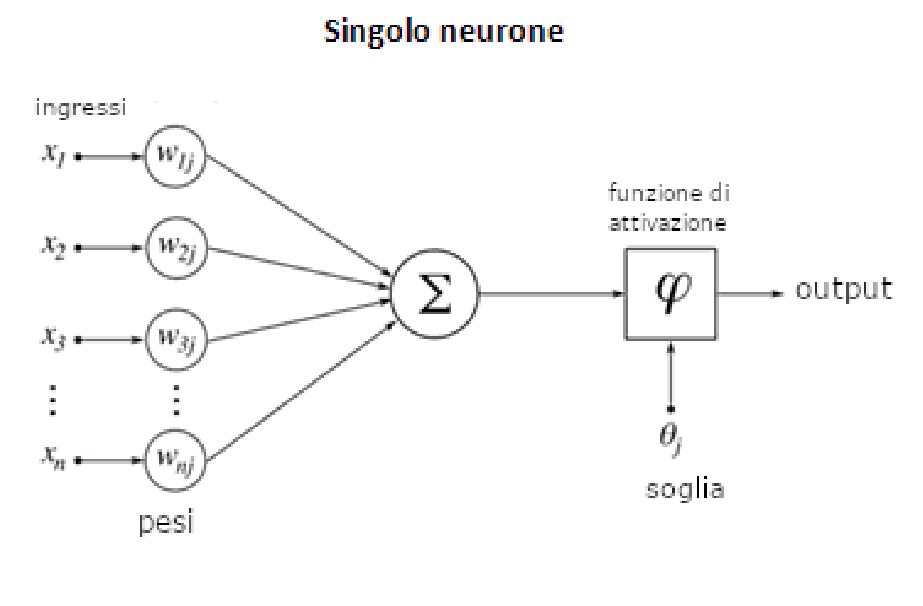
\includegraphics[scale=0.8]{neurone.eps}
\caption{Modello non lineare di un neurone artificiale.}
\label{neurone}
\end{figure}
\newpage
La figura \ref{neurone}, indipendentemente dal modello di rete utilizzato, mostra l'elaborazione eseguita da un neurone artificiale.\\
Siano $x_1,\cdots,x_n$ i dati in input, rappresentati dagli $n$ nodi del primo strato, nel k-esimo neurone l'informazione viene elaborata come:
$$y_{(k)}=f(b_{(k)}+\sum_{i=1}^n w_{(k)i}\cdot x_{(k-1)i})$$
dove:\\
\begin{itemize}
\item $y_{(k)}$ \`e l'output generato dal neurone k;
\item $b_{(k)}$ \`e il valore soglia del neurone k;
\item $w_{(k)i}$ \`e il peso associato all'arco che collega il nodo i-esimo al neurone $k$;
\item $f(\cdot)$ \`e la funzione di attivazione.
\end{itemize}
Il motivo principale per cui vengono scelte le reti neurali \`e la possibilit\'{a} di parallelizzare i calcoli.
\newpage
\section{Funzioni di attivazione}
La funzione di attivazione \`e una funzione usata per normalizzare, quindi limitare, l'ampiezza dell' output, per non consumare eccessiva memoria e di velocizzare il processo di calcolo.\\
Generalmente le reti neurali sono utilizzate per implementare funzioni complesse e le funzioni di attivazione non lineari consentono loro di approssimare funzioni arbitrariamente complesse. Le funzioni maggiormente utilizzate a tale scopo sono 3:
\begin{figure}[!h]
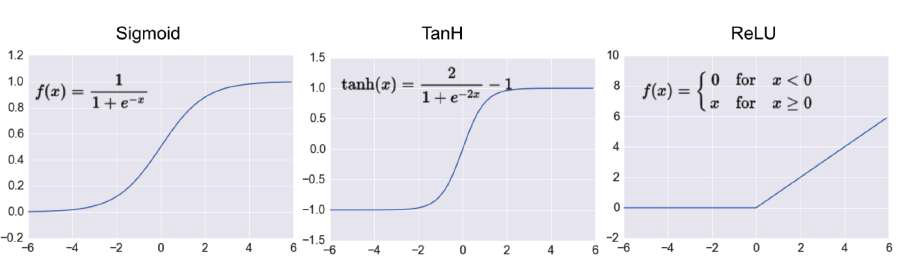
\includegraphics[scale=0.7]{funzioniAttivazione}
\caption{Grafici delle funzioni di attivazione pi\`{u} usate.}
\end{figure}

\subsubsection{Sigmoid}
La funzione Sigmoid viene usata sopratutto nei modelli in cui si deve prevedere la probabilit\`{a} come output, poich\'{e} il suo codominio \`e l'intervallo: $(0,1)$ ed \`e definita come:
$$S:\mathbb{R}\longrightarrow(0,1)$$
$$S(x)=\frac{1}{1+e^{-x}}$$
La Sigmoid \`e una funzione monotona e differenziabile, infatti la sua derivata:
$$\frac{dS}{dx}=\frac{e^{-x}}{(1+e^{-x})^2}$$
\`e continua, positiva e derivabile in  ogni punto del dominio.
\subsubsection{tanh}
La funzione tangente iperbolica \`e definita come: $$\tanh:\mathbb{R}\longrightarrow(-1,1)$$ 
$$ \tanh(x)=\frac{2}{1+e^{-2x}} - 1$$ 
\`e simile alla Sigmoide, infatti sono legate dalla relazione:
$$
\tanh(x)=2 \cdot S(2x)-1
$$
ma ha un intervallo di output pi\`{u} ampio, che le consente di produrre anche output di segno negativo. Anche questa funzione \`e monotona e differenziabile.\\
Purtroppo essendo funzioni limitate, per valori alti tendono ad un valore specifico: $$\lim_{x \to +\infty} \tanh(x)=1$$
Questo comportamento pu\`{o} portare ad una perdita di informazioni: se $x$ corrisoponde ad un valore elevato e subisce una grande variazione, per la funzione invece avr\`{a} subito una variazione minima.\\
Lo stesso problema si presenta con le derivate, provocando la "scomparsa del gradiente"(\textit{vanishing gradient}), fondamentale per approssimare al meglio la funzione; ma questo argomento verr\`{a} affrontato in \ref{back-prop}.
\subsubsection{ReLu}
La funzione ReLu (Rectified Linear Unit) \`e la funzione pi\'{u} utilizzata nel deep learning e, in particolare, nelle reti convoluzionali. \`{E} definita:
$$Relu:\mathbb{R}\longrightarrow [0,\infty)$$
$$
Relu(x)=
\left\{
\begin{array}{rl}
x & \mbox{se } x \geq 0 \\
0 & \mbox{se } x < 0
\end{array}
\right.
$$
Sia la funzione, che la sua derivata sono monotone. A differenza delle funzioni precedenti, la sua derivata \`e molto semplice da calcolare:
$$
Relu^{\prime}(x)=
\left\{
\begin{array}{rl}
1 & \mbox{se } x \geq 0 \\
0 & \mbox{se } x < 0
\end{array}
\right.
$$
e non rischia di incorrere nella sparizione del gradiente. Si potrebbero avere problemi nell'origine, per la presenza di un punto angoloso, poich\'{e} la derivata \`e indefinita ma, per convenzione, viene definita uguale a zero.\\
Risulta immediato il motivo per cui sono molto utilizzate nelle reti formate da tanti strati: mappando i valori negativi in zero, permette di tenere solo i valori positivi, riducendo di molto il numero di neuroni attivati.

\section{Addestramento di una rete}
Come visto in \ref{Costruzione}, per addestrare un algoritmo si ha bisogno di una funzione di perdita e di un metodo per minimizzare l'errore di valutazione.\\
L'addestramento di una rete neurale si basa sugli stessi principi:\\
si definisce una mappa: $$y=f(x,\theta)$$ e si cerca il valore del parametro $\theta$ che pi\`{u} accuratamente approssima la funzione.
Bisogna quindi trovare dei parametri che minimizzano la funzione di perdita:
$$L[y,f^*(x,\theta)]$$
ovvero, trovare $\hat{\theta}$ tali che:
$$\hat{\theta}=\argmin_{\theta} \left\{ \frac{1}{n} \sum_{i=1}^{n} L[y_i,f^*(x_i,\theta)] \right\}$$
Questo processo \`e necessario per approssimare una determinata funzione $f^*$, che descrive il comportamento della rete.\\
Durante l'addestramento, la rete viene provata pi\`{u} volte, ogni volta con un input diverso, fino a che l'errore di addestramento \`e molto piccolo. In questa fase, ad ogni iterazione viene passato in input un insieme di addestramento, viene fissato un valore $\theta_{0}$ iniziale, e tramite la funzione di perdita, si calcola l'errore di addestramento. In questo modo la rete ha il valore di quanto ciascun neurone di output sia lontano dal proprio valore atteso, e in che direzione (positiva o negativa).\\
Per esempio, nel caso di riconoscimento dei numeri scritti a mano (MNIST):
se il risultato atteso \`e 6, nell'output ci aspettiamo che nella posizione corrispondente al sesto neurone ci sia il valore 1 e 0 in tutti gli altri. Se al neurone 6 \`e associato il valore $0.7$, allora la correzione da fare \`e di 0.3. Quindi la rete ripete l'addestramento aggiornando il peso corrispondente al neurone valutato con $\theta_{1}$ e cos\'{i} via, fino a che il valore corrispondente al neurone 6 \`e molto vicino a 1. Viceversa, se il neurone 4 invece di 0 presenta 0.8, allora la correzione sar\'{a} -0.8 e si aggiorneranno i pesi relativi a questo neurone in modo da abbassarne drasticamente l'output.\\
L'algoritmo appena descritto a parole prende il nome di \textit{back propagation}.
\newpage
\subsubsection{Algoritmo di back propagation}\label{back-prop}
Si consideri una rete neuronale composta da L strati, dove l'output \`e composto da un valore solamente.
L'algoritmo di back propagation si divide in due fasi:
\begin{itemize}
\item propagazione in avanti (\textit{forward propagation});
\item propagazione all'indietro (\textit{backward propagation})
\end{itemize}
\textbf{Forward propagation}
Durante la propagazione in avanti, si calcolano tutti i valori dei nodi presenti nella rete $a_{i}^k$:
\begin{equation}\label{eqbp0}
a_{i}^{k}=b_{i}^{k}+\sum_{j=1}^{r_{k-1}} w_{ji}^{k}\cdot o_{j}^{k-1}
\end{equation}
dove:
\begin{itemize}
\item $w_{ij}^{k}$ \`e il peso associato all'arco che collega il nodo i del k-esimo strato con il nodo j;
\item $b_{i}^{k}$ \`e il valore soglia del nodo i nel k-esimo strato;
\item $o_{i}^{k}$ \`e l'output del nodo i nel k-esimo strato;
\item $r_k$ \`e il numero di nodi presenti nel k-esimo strato.
\end{itemize}
Calcolato l'ultimo valore $a^{L}$, corrispondente all'output della rete, si esamina l'errore di allenamento tramite la funzione di perdita. Per minimizzare l'errore, basta minimizzare la funzione di perdita, questa operazione sancisce l'inizio della seconda fase: la backward propagation.\\
\textbf{backward propagation}
Per ottenere il minimo di una funzione bisogna vedere dove si annulla la sua derivata prima. Trattandosi di una funzione a pi\`{u} variabili, si dovr\`{a} calcolare il gradiente della funzione di perdita: $L[y,f(x,\theta)]$, per farlo  si applica la regola della catena per il calcolo e poich\'{e} $\theta = (W^1,W^2,\cdots ,W^{L-1})$, abbiamo:
\begin{equation}\label{eqbp1}
\frac{\partial L}{\partial w_{ij}^k}=\frac{\partial L}{\partial a_j^k}\frac{\partial a_j^k}{\partial w_{ij}^k}.
\end{equation}
Il punto di forza di questo algoritmo consiste nell'introdurre una quantit\'{a} di costo (anche chiamata errore):
\begin{equation}\label{eqbp2}
\delta_j^k\equiv \frac{\partial L}{\partial a_j^k}
\end{equation}
attraverso la quale si calcolano le derivate parziali in modo iterativo, ripercorrendo la rete all'indietro.\\
Dall'eq \ref{eqbp0} si ricava:
\begin{equation}
\frac{\partial a_j^k}{\partial w_{ij}^k}=\frac{\partial}{\partial w_{ij}^k}\left( \sum_{l=0}^{r_{k-1}}w_{lj}^k o_l^{k-1}\right)=o_i^{k-1}
\end{equation}
sostituendola nell'eq \ref{eqbp1} si ottiene:
\begin{equation}
\frac{\partial L}{\partial w_{ij}^k}=\delta_j^k o_i^{k-1}
\end{equation}
Partendo dallo strato dell'output, considerando come funzione di perdita: $$L=\frac{1}{2}(\hat{y}-y)^2=\frac{1}{2}(g_o(a^L)-y)^2,$$
si ha che:
\begin{equation}
\delta^{L}=(g_o(a^L)-y)g_o^{\prime}(a^L)=(\hat{y}-y)g_o^{\prime}(a^L).
\end{equation}
dove $g_o$ \`e la funzione di perdita per l'output.\\
Quindi la derivata parziale della funzione di perdita \`e:
\begin{equation}
\frac{\partial L}{\partial w_{iL-1}^L}=\delta^L o_i^{L-1}
\end{equation}
Per gli strati nascosti invece abbiamo:
\begin{equation}\label{eqbp3}
\delta_j^k=\sum_{l=1}^{r_{k+1}}\frac{\partial L}{\partial a_l^{k+1}}\frac{\partial a_l^{k+1}}{a_j^k}=\sum_{l=1}^{r_{k+1}} \delta_l^{k+1} \frac{\partial a_l^{k+1}}{a_j^k},
\end{equation}
Sostituendo in \ref{eqbp3} la \ref{eqbp0} e denotando con $g$ la funzione di perdita dello strato nascosto, si ottiene la formula di propagazione all'indietro:
\begin{equation}
\delta_j^k=g^{\prime}(a_j^k)\sum_{l=1}^{r_{k+1}}w_{jl}^{k+1}\delta_l{k+1}
\end{equation} 
e la derivata parziale della funzione di perdita, rispetto ai pesi degli strati nascosti $w_{ij}^{k+1}$ , $1\leq k < L$, si ottiene con:
\begin{equation}
\frac{\partial L}{\partial w_{ij}^k}=\delta_j^k o_i^{k-1}=g^{\prime}(a_j^k)o_i^{k-1}\sum_{l=1}^{r_{k+1}}w_{jl}^{k+1}\delta_l{k+1}
\end{equation}
Ora pu\'{o} avvenire l'aggiornamento dei pesi tramite il metodo SGD (Stochastic Gradient Descent), ovvero in formule:
\begin{equation}\label{eqbp4}
w_{ij}^{k+1}=w_{ij}^k + \eta \frac{\partial L}{\partial w_{ij}}
\end{equation}
dove $\eta \in (0,1]$ rappresenta il fattore di apprendimento (\textit{learning rate}).\\
La scelta del fattore di apprendimento influenza molto il comportamento dell'algoritmo in quanto, se si scelgono valori troppo piccoli la convergenza sar\`{a} lenta, mentre se si scelgono valori troppo grandi si rischia di avere una rete instabile con comportamento oscillatorio.\\
Un metodo semplice per incrementare il fattore di apprendimento, senza il rischio di rendere la rete instabile, \`{e} quello di modificare la regola di aggiornamento inserendo nell'equazione \ref{eqbp4} un ulteriore parametro $\alpha$ (detto momento), ottenendo:
\begin{equation}
w_{ij}^{k+1}=\alpha w_{ij}^k + \eta \frac{\partial C}{\partial w_{ij}}.
\end{equation}
Se si espande ricorsivamente la formula si ottiene:
\begin{equation}
w_{ij}^{k+1}=\eta \sum_{l=1}{k+1}\alpha_{k+1-l}\frac{\partial L}{\partial w_{ij}^l}
\end{equation}
Inserendo il momento si ha il vantaggio che se la derivata parziale tende a mantenere lo stesso segno su iterazioni consecutive, grazie alla sommatoria, l'aggiornamento produce valori pi\'{u} ampi e quindi tende ad accelerare nelle discese del gradiente. Se invece la derivata ha segni opposti ad iterazioni consecutive, la sommatoria tende a diminuire l'ampiezza dell'aggiornamento, in questo modo non si corre il rischio di avere dei loop infiniti nel caso di minimi locali della funzione d'errore.\\
A tal proposito generalmente i criteri di arresto dell'algoritmo possono essere:
\begin{itemize}
\item $\lVert \nabla L\rVert < \epsilon$
\item $L[y,f(x,\theta)]=0$;
\item $L_i[y,f(x,\theta_i)]-L_j[y,f(x,\theta_j)]<<\epsilon^{\prime}$
\end{itemize}
dove $L_i$ e $L_j$ sono due epoche consecutive. Un'epoca corrisponde alle due fasi di propagazione necessarie per un aggiornamento dei pesi.
\subsection*{Il problema del Vanish Gradient}
Come accennato in precedenza, l'uso del metodo del gradiente va applicato con attenzione e parametri adatti, altrimenti si incorre nel fenomeno detto "sparizione del gradiente", ovvero del \textit{vanish gradient}.\\
Si ipotizzi di avere una rete profonda semplice, ovvero con 3 livelli nascosti e con un solo neurone in ogni strato:

\begin{figure}[!h]
\centering
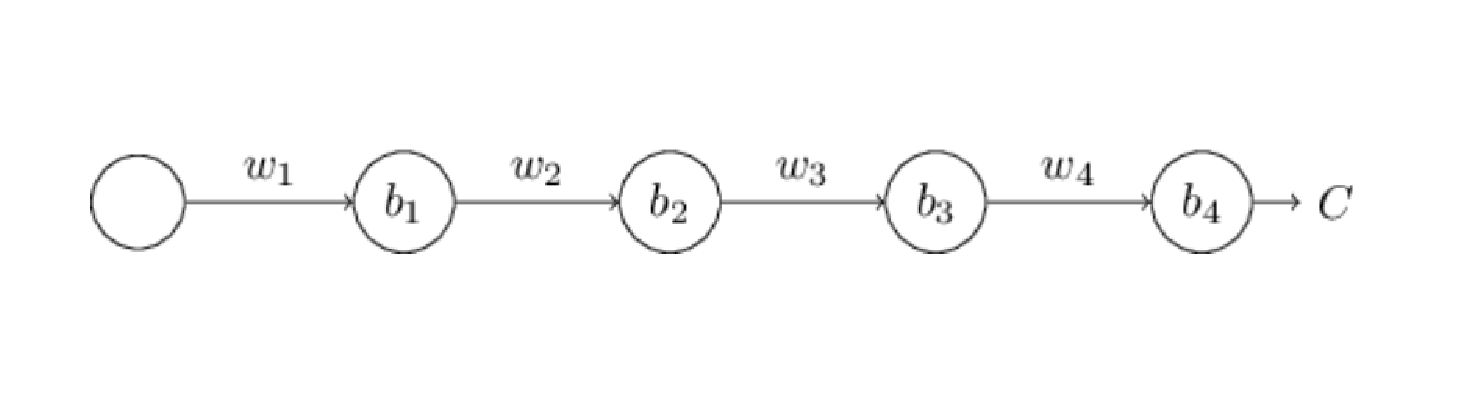
\includegraphics[scale=0.5]{vanish}
\caption{Rete neurale semplice costituita da 3 strati con: $w_j$ pesi, $b_j$ i valori soglia e C funzione di costo.}
\label{fig:vanish}
\end{figure}

Applicando l'eq \ref{eqbp0} per il calcolo dell'output di un nodo, alla rete rappresentata in figura \ref{fig:vanish}, si ottiene:
\begin{equation}
a_j=\sigma(w_j a_{j-1} +b_j)
\end{equation}
dove $\sigma$ \`e la funzione di attivazione Sigmoid.\\
Si pone $z_j=w_j a_{j-1} +b_j$ e si ottengono le seguenti relazioni:
\begin{eqnarray}
a_4&=&\sigma(z_4)\nonumber \\
z_4&=&w_4 \sigma(z_3)+b_4 \nonumber \\
z_3&=&w_3 \sigma(z_2)+b_3 \nonumber \\
z_2&=&w_2 \sigma(z_1)+b_2 \nonumber \\
z_1&=&w_1 \sigma(z_0)+b_1 \nonumber
\end{eqnarray}
Si \`e indicato con C una funziona di costo, per sottolineare che il costo \`e una funzione dell'output della rete (in questo caso $a_4$).\\
Se C ha un valore basso l'output sar\'{a} vicino a quello desiderato, viceversa per alti valori di C l'output calcolato si allontaner\'{a} dal risultato che ci si auspicava.\\
Il gradiente associato al primo strato viene calcolato applicando la regola della catena:
\begin{equation} \label{catena}
\frac{\partial C}{\partial b_1}=\frac{\partial C}{\partial a_4} \cdot \frac{\partial a_4}{\partial a_3} \cdot \frac{\partial a_3}{\partial a_2} \cdot \frac{\partial a_2}{\partial a_1} \cdot \frac{\partial a_1}{\partial b_1}
\end{equation}
Calcoliamo singolarmente ogni elemento dell'equazione:
\begin{equation}
\frac{\partial a_1}{\partial b_1} = \frac{\partial \sigma (z_1)}{\partial b_1} = \frac{\partial \sigma(w_1 \sigma(z_0)+b_1)}{\partial b_1} = \sigma '(z_1)
\end{equation}
\begin{equation}
\frac{\partial a_2}{\partial a_1}=\frac{\partial \sigma (z_2)}{\partial a_1} = \frac{\partial \sigma(w_2 a_1 +b_2)}{\partial a_1} = w_2 \sigma ' (z_2)
\end{equation}
\begin{equation}
 \frac{\partial a_3}{\partial a_2}=\frac{\partial \sigma (z_3)}{\partial a_2} = \frac{\partial \sigma(w_3 a_2 +b_3)}{\partial a_2} = w_3 \sigma ' (z_3)
\end{equation}
\begin{equation}
 \frac{\partial a_4}{\partial a_3}=\frac{\partial \sigma (z_4)}{\partial a_3} = \frac{\partial \sigma(w_4 a_3 +b_4)}{\partial a_3} = w_4 \sigma ' (z_4)
\end{equation}
Quindi l'eq \ref{catena} diventa:
\begin{equation}\label{eqstima}
\frac{\partial C}{\partial b_1}= \frac{\partial C}{\partial a_4} w_4 \sigma ' (z_4) w_3 \sigma ' (z_3) w_2 \sigma '(z_2) \sigma '(z_1).
\end{equation}
Si noti che l'equazione \ref{eqstima} \`e il prodotto di termini della forma: $w_j  \sigma '(z_j)$, fatta eccezione per il primo termine.\\
Tipicamente, i valori iniziali dei pesi vengono ricavati dai valori che pu\'{o} assumere una distribuzione normale avente media 0 e deviazione standard 1, allora: $$|w_j|<1,\qquad \forall j.$$
La derivata raggiunge il massimo in 0: $\sigma '(0)=\frac{1}{4}$, quindi ogni termine dell'equazione \`e tale che $$|w_j \sigma '(z_j)| < \frac{1}{4}, \qquad \forall j,$$ si ottiene la stima del tipo:
\begin{equation}
\frac{\partial C}{\partial b_1}= \frac{\partial C}{\partial a_4} \underbrace{w_4 \sigma '(z_4)}_{<\frac{1}{4}} \underbrace{w_3 \sigma '(z_3)}_{< \frac{1}{4}} \underbrace{w_2 \sigma '(z_2)}_{< \frac{1}{4}}\underbrace{\sigma '(z_1)}_{< 1} \nonumber
\end{equation}
\begin{figure}[!h]
\centering
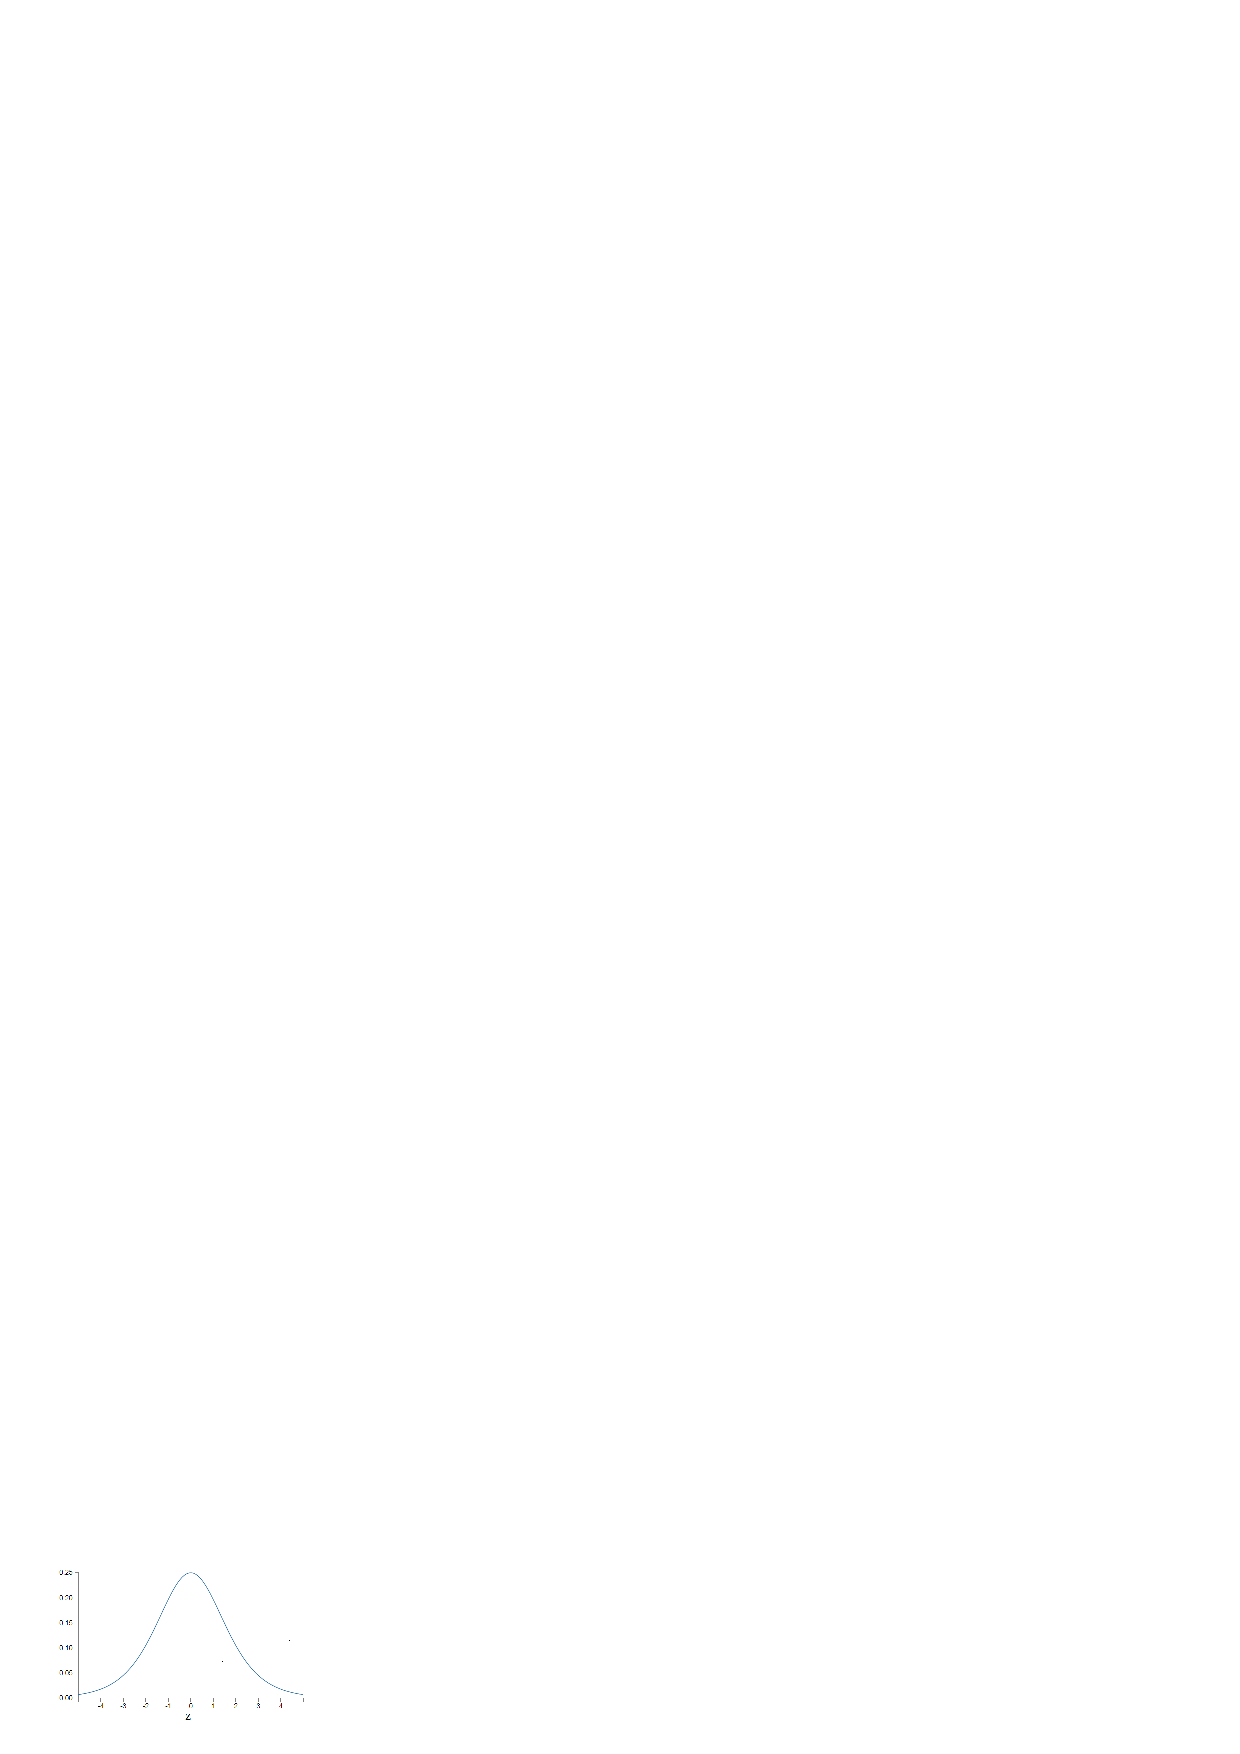
\includegraphics[scale=2]{derivataSigmoid}
\caption{Grafico della funzione $\sigma '(z)$}
\end{figure}
\newpage
Questo comportamento implica che, con l'aumentare della profondit\'{a} della rete, il valore del gradiente tende a diminuire di un fattore di $\frac{1}{4}$ per ogni strato, fino a tendere a 0 prematuramente; ovvero a "scomparire" da un certo strato in poi.\\
L'utilizzo della funzione di attivazione ReLu risolve il problema, grazie alla sua caratteristica di avere il gradiente sempre pari a 1. Questo comporta che , non solo il gradiente non subisce una diminuzione progressiva in ogni strato, ma mantiene il suo valore inalterato.\\
Si ricorda che $ReLu(z)=z_{+}=max(0,z)$, il che comporta che alcuni neuroni non vengono attivati e quindi non influenzeranno in alcun modo l'algoritmo scelto per individuare i pesi ottimali per la rete.\\
Ne consegue che  $ReLu'(z)=1$ per ogni nodo rimasto attivo.\\
Nel caso della rete prima analizzata con la funzione Sigmoid, si \`e dovuta fare una stima del gradiente per ogni neurone, con l'inserimento della ReLu non \`e necessario e il calcolo del gradiente \`e:
\begin{equation}
\frac{\partial C}{\partial b_j}=1, \qquad \forall j.
\end{equation}
\begin{figure}[!h]
\centering
\caption{Grafico di $ReLu'(z)$}
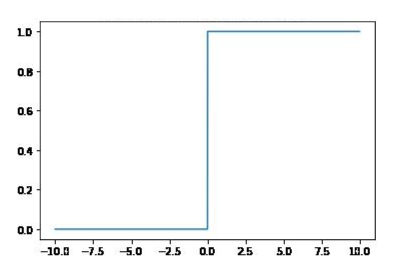
\includegraphics[scale=1.8]{derivataRelu}
\end{figure}
\newpage
\section{Reti Deep Feed-forward}
Le reti Feed-forward sono le reti neurali profonde con la struttura pi\`{u} semplice, composte da almeno uno strato nascosto. La loro struttura \`e rappresentata da un grafo aciclico diretto in un'unica direzione, dove ogni nodo di uno strato \`e connesso con tutti i nodi dello strato successivo e nessun nodo \`e connesso con un nodo appartanente allo stesso strato.
\begin{figure}[!h]
\centering
\includegraphics[scale=0.37]{network-neurale}
\caption{modello di rete deep feedforward con uno strato}\label{rete}
\end{figure}

Questo tipo di reti sono di solito rappresentate dalla composizione di pi\`{u} funzioni, dal momento che l'output di un nodo non pu\'{o} essere passato in input ad una funzione gi\`{a} eseguita. Nel caso di una rete con L strati avremo che  la relazione che lega il vettore di input $x$ con quello di output $y$ risulta essere:
\begin{equation}
y=f(x,\theta)=g_o(\theta_{L-1}g_{L-1}(\cdots \theta_{2}g_{2}(\theta_{1}x)))
\end{equation}
Lo scopo della rete \`e sempre di approssimare $f(x)$ ad una funzione $f^*$ e questo \`e possibile grazie all'addestramento.

\section{ImageNet}\label{ImageNet}
In Internet oramai sono presenti milioni di milioni di immagini e di video, usati per i modelli e gli algoritmi pi\'{u} sofisticati e robusti, per aiutare gli utenti ad indicizzare, recuperare, organizzare e interagire con questi dati.
Un esempio banale \`e la ricerca di immagini su Google.\\
Se si volesse ricercare una razza canina in particolare, come fa l'algoritmo ad individuare un'immagine di un Labrador piuttosto che di un Beagle?\\
Lo fa tramite categorie e sottocategorie. Ma esattamente come tali dati possono essere utilizzati e organizzati \`e un problema che non \`e ancora stato risolto.\\
Di solito i motori di ricerca possono trovare una determinata immagine solo se il testo inserito corrisponde al testo con cui \`e stato etichettato. Ma le etichette possono essere inaffidabili, inutili (nel caso di dialetti e nomignoli) o semplicemente inesistenti.\\
Si vuole quindi cercare un metodo per far imparare alle macchine come riconoscere oggetti simili che non sono stati ancora etichettati, rendendo possibile un notevole aumento dell'accuratezza del riconoscimento.\\
\`{E} stato creato \textit{ImageNet}: un grande database visivo contenente oltre 14 milioni di immagini etichettate, progettato per l'utilizzo nella ricerca di software per il riconoscimento di oggetti visivi.\\
ImageNet si basa sulla struttura gerarchica fornita da un altro database: \textit{WordNet}. WordNet \`e un database semantico-lessicale per la lingua inglese elaborato dal linguista George Armitage Miller presso l'Universit\'{a} di Princeton, che si propone di organizzare, definire e descrivere i concetti espressi dai vocaboli. L'organizzazione del lessico si avvale di raggruppamenti di termini con significato affine, chiamati \textit{"synset"} (dalla contrazione di synonym set) e del collegamento dei loro significati attraverso diversi tipi di relazioni chiaramente definite. All'interno dei synset le differenze di significato sono numerate e definite.\cite{wordnet}\\
%chiedere se devo specificare che questa � la grafica bitmap%
Un'immagine digitale \`e formata da diversi quadratini disposti in modo regolare su una griglia di punti equidistanti. Questi quadratini sono detti \textit{pixel (picture elements)}.\\
I pixel presenti in um'immagine ne determinano la dimensione e la risoluzione; ad esempio un'immagine di dimensione $320 \times 240$ pixel indica che sono presenti 240 pixel orizzontali e 320 verticali. Pi\'{u} i pixel sono numerosi, e quindi pi\'{u} piccoli e fitti, pi\'{u} la risoluzione \`e alta.\\
In ogni pixel risiede un'informazione espressa in bit riguardante (generalmente) il colore: un pixel da 1 bit pu\'{o} avere solo $2^1$colori (generalmente il bianco e il nero), mentre uno da 1 byte (8bit)  pu\'{o} rappresentare $2^8=256$ colori. Il numero di colori possibili \`e detto anche profondit\'{a}. Le rappresentazioni delle immagini a colori variano a seconda dei campi di colore che si usano, solitamente, ogni campo viene rappresentato da 1 byte e rappresenta il livello di intensit\'{a} dei colori fondamentali.\\
Il modello pi\'{u} utilizzato \`e quello RGB, dove per ogni pixel vengono utilizzati 3 byte:
\begin{itemize}
\item 1 byte per la componente rossa (R)
\item 1 byte per la componente verde (G)
\item 1 byte per la componente blu (B)
\end{itemize}
ma ne esistono anche altri come, ad esempio, CMYK che considera come colori fondamentali: ciano, magenta, giallo e nero.\\
Tipicamente nel dataset di ImageNet la dimensione media delle immagini \`e di circa $400 \times 350$ pixel.
\section{Reti Neurali Convoluzionali - CNNs}
Le reti neurali convoluzionali (\textit{Convolutional Neural Networks}) sono un tipo particolare di reti neurali a strati che usano, in almeno uno dei loro strati, la convoluzione al posto della classica moltiplicazione tra matrici.
\begin{defin}
Siano $f,g\in L^1(\mathbb{R})$, si definisce convoluzione tra f e g come:
\begin{equation}\label{eqconvoluzione}
(f*g)(t):= \int_{-\infty}^{\infty} f(\tau)g(t-\tau)d\tau=y(t)
\end{equation}
\end{defin}
Questa operazione gode di alcune propriet\'{a}:
\begin{enumerate}
\item \textbf{propriet\'{a} commutativa} \begin{eqnarray}
(f*g)(t)& := & \int_{-\infty}^{\infty} f(\tau)g(t-\tau)d\tau=-\int_{\infty}^{-\infty} f(t-z)g(z)dz=\nonumber \\
& = & \int_{-\infty}^{\infty}g(z)f(t-z)dz=(g*f)\end{eqnarray}
dove $z=t-\tau \Rightarrow \tau=t-z \Rightarrow d\tau=-dz$.
\item \textbf{Linearit\'{a}}$$ (f_1+f_2)*g=(f_1*g)+(f_2*g), \qquad (\lambda f)*g=\lambda(f*g).$$ 
\item \textbf{Integrale} Se $f,g\in L^1(\mathbb{R})$ sono assolutamente integrabili allora $$\int_{\mathbb{R}}(f*g)(t)dt=\int_{\mathbb{R}}f(t)dt \cdotp \int_{\mathbb{R}}g(t)dt.$$
\item \textbf{Cambiamenti di scala} $$se y=f*g\Rightarrow f(\lambda t)*g(\lambda t)=\frac{1}{|\lambda|}y((\lambda t)$$
\item \textbf{Derivate} Se f  \`e regolare a tratti e continua, allora 
$$ \frac{d}{dt}(f*g)(t)=\frac{d}{dt}f(t)*g(t)=f(t)*\frac{d}{dt}g(t)$$
\item \textbf{Supporti} Se supp $f\subset [a,b]$ e supp $g\subset [c,d]\Rightarrow $\\
$\Rightarrow$ supp $(f*g)\subset [a+c,b+d].$
\item \textbf{Segnali causali} Se f,g sono causali $\Rightarrow f*g$ \`e causale.
\end{enumerate}
Tramite l'eq. \ref{eqconvoluzione}, se si conosce la funzione di risposta g(t) e il segnale di entrata f(t), si pu\`{o} esprimere il segnale di uscita y(t), che nelle reti convoluzionali rappresenta il filtro di convoluzione (\textit{feature map}) e la funzione di risposta \`e detta \textit{"kernel"}.
Si ricorda che per \textit{segnale} si intende una grandezza fisica qualsiasi a cui \`e associata un'informazione.\\
Nelle reti neurali i segnali non sono descritti da funzioni continue ma da funzioni discrete, in quanto l'input passato ad un neurone \`e un valore discreto ben preciso.\\
Si necessita qundi delle seguenti definizioni:
\begin{defin}
I \textit{segnali discreti} sono definiti come funzioni di variabili indipendenti che possono assumere solo un insieme finito di valori discreti.\\
Un segnale discreto nel tempo x, consiste in una sequenza di numeri indicata con 
$$x_n \qquad oppure \qquad x(n) ,\quad n\in \mathbb{Z}$$
\end{defin}
\begin{defin}
Siano $f(n)$ e $g(n)$ due sequenze, si definisce la loro convoluzione discreta come:
\end{defin}
\begin{equation} \label{eqconvoluzionediscreta}
f(n)*g(n)=\sum_{k=-\infty}^{\infty}x(k)g(n-k)=y(k)
\end{equation}
Valgono le stesse propriet\'{a} prima citate per la convoluzione nel caso continuo. Nel nostro problema di analisi di immagini, data un'immagine di dimensione M $\times$ N pixel l'eq\ref{eqconvoluzionediscreta} diventa:
\begin{equation}
(f*g)(x,y)=\sum_{i=0}^M \sum_{j=0}^N f(x,y)g(x-i,y-j)
\end{equation}
La caratteristica principale per cui le reti convoluzionali sono maggiormente indicate per l'elaborazione di immagini \`e la loro struttura, basata sull'elaborazione di dati nella forma di array multipli.\\
Come descritto nel paragrafo \ref{ImageNet} \`e facilmente intuibile come ogni dimensione caratterizzante un'immagine pu\'{o} essere vista come un array multidimensionale, ovvero un tensore.\\
I neuroni di ciascun livello sono organizzate in griglie o volumi 3D.\\
L'altezza e la larghezza rappresentano i pixel, mentre la profondit\`{a} le caratteristiche dell'oggetto, chiamate \textit{feature map}.
\begin{figure}[!h]
\centering
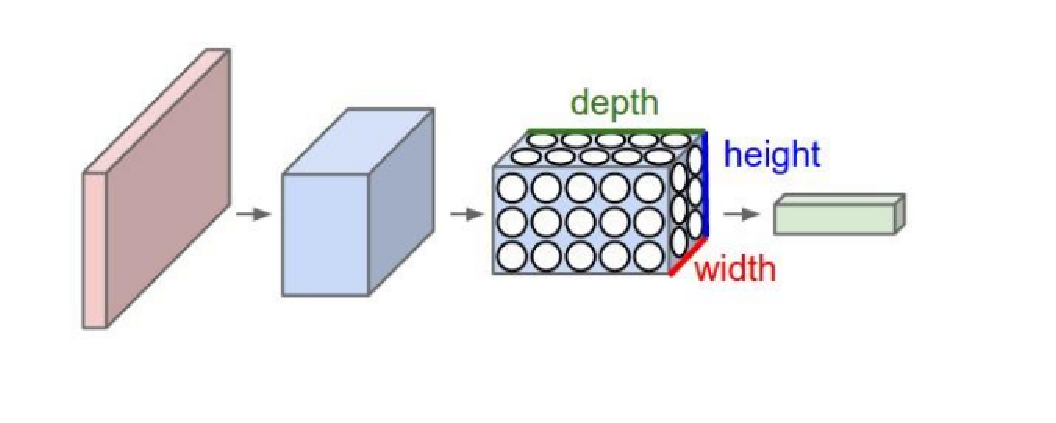
\includegraphics{Immagine3D}
\caption{Esempio di rappresentazione di un'immagine in formato RGB in una CNN.}
\end{figure}
\newpage
\subsection{Struttura di una CNNs}
Alla base di questa tipologia di reti neurali ci sono 3 concetti:
\begin{enumerate}
\item connettivit\`{a} locale (\textit{sparse interactions})
\item condivisione dei parametri
\item alternanza di strati di convoluzione e di \textit{pooling}
\end{enumerate}
La \textbf{connettivit\`{a} locale} consiste nello sfruttare le correlazioni spaziali presenti all'interno dei dati di input e viene applicata tra neuroni di strati adiacenti. Questo \`e possibile applicando un kernel pi\`{u} piccolo dell'input che, tramite l'operazione di convoluzione, dar\`{a} in output un numero minore di neuroni. Ne consegue una forte riduzione del numero di connessioni tra i nodi della rete.\\
Nelle prossime sezioni sar\`{a} pi\`{u} chiaro cosa questo voglia dire, ma se si considera, ad esempio, un'immagine e su di essa ci si focalizzi su un singolo pixel, in base alle correlazioni con i pixel circostanti si possono ricavare informazioni locali sull'immagine (ad esempio bordi, colori, forme geometriche, ecc...).\\
Attraverso la \textbf{condivisione dei parametri} si utilizza lo stesso parametro per pi\'{u} di una funzione in un modello, permettendo alla rete di apprendere un insieme di parametri invece che insiemi separati di parametri per ogni posizione, questo comporta che l'algoritmo deve tenere in memoria un numero minore di parametri.\\
\begin{figure}[!h]
\centering
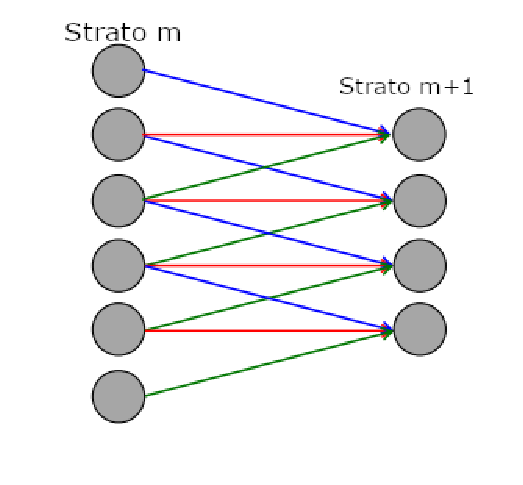
\includegraphics{CNN}
\caption{Ciascuno dei 4 neuroni a destra \`{e} connesso solo a 3 neuroni del livello precedente. I pesi sono condivisi (stesso colore stesso peso).}
\end{figure}
\\Nella figura precedente si pu\`{o} notare che sono presenti in totale 12 connessioni (3$\times$ 4) e 3 pesi, mentre in una normale rete neurale equivalente avremmo avuto 24 connessioni (6 $\times$ 4) e 24 pesi. In un solo livello sono state utilizzate la met\`{a} delle connessioni e $\frac{1}{8}$ dei pesi.
\newpage
L'architettura di una rete convoluzionale \`e formata, tipicamente, da tre tipi di strati:
\begin{enumerate}
\item convoluzionali;
\item pooling;
\item totalmente connessi.
\end{enumerate}
Uno strato tipico di una rete convoluzionale consiste di tre fasi .Nella prima fase lo strato esegue diverse convoluzioni in parallelo per produrre un set di attivazioni lineari. Nella seconda fase, ogni attivazione lineare viene eseguita attraverso una funzione di attivazione non lineare. Nella terza fase, si esegue  una funzione di  pooling per modificare ulteriormente l'output dello strato.
\subsubsection{Strati convoluzionali}
Lo scopo dello strato convoluzionale (\textit{convolutional layer}) \`e quello di rilevare delle particolari caratteristiche all'interno di un oggetto, grazie ad un'analisi locale. Questo compito \`e affidato al kernel della convoluzione, detto anche filtro, che si comporta come una finestra bidimensionale composta da pesi che scorre su tutto l'input. Di ogni porzione di input viene calcolata la sua convoluzione con il kernel, producendo cos\`{\i} un output di dimensioni ridotte rispetto all'input. Questo output viene chiamato \textit{feature map} e racchiude le caratteristiche che il filtro cercava ed \`e qui che i pesi sono condivisi: i neuroni di una stessa feature map processano porzioni diverse dell' input nello stesso modo.\\
Il kernel ha due iperparametri, chiamati passo(\textit{stride}) e dimensione(\textit{size}). La size  pu\`{o} essere qualsiasi dimensione di un rettangolo, mentre lo stride \`e il numero di pixel che si fanno scorrere tra due computazioni della finestra di kernel. Se lo stride ha lunghezza 1, il filtro si sposta di un pixel alla volta, se ha lunghezza 2, i filtri saltano 2 pixel alla volta durante lo scorrimento, producendo un'immagine con dimensione dimezzata.

\begin{figure}[!hb]
\centering
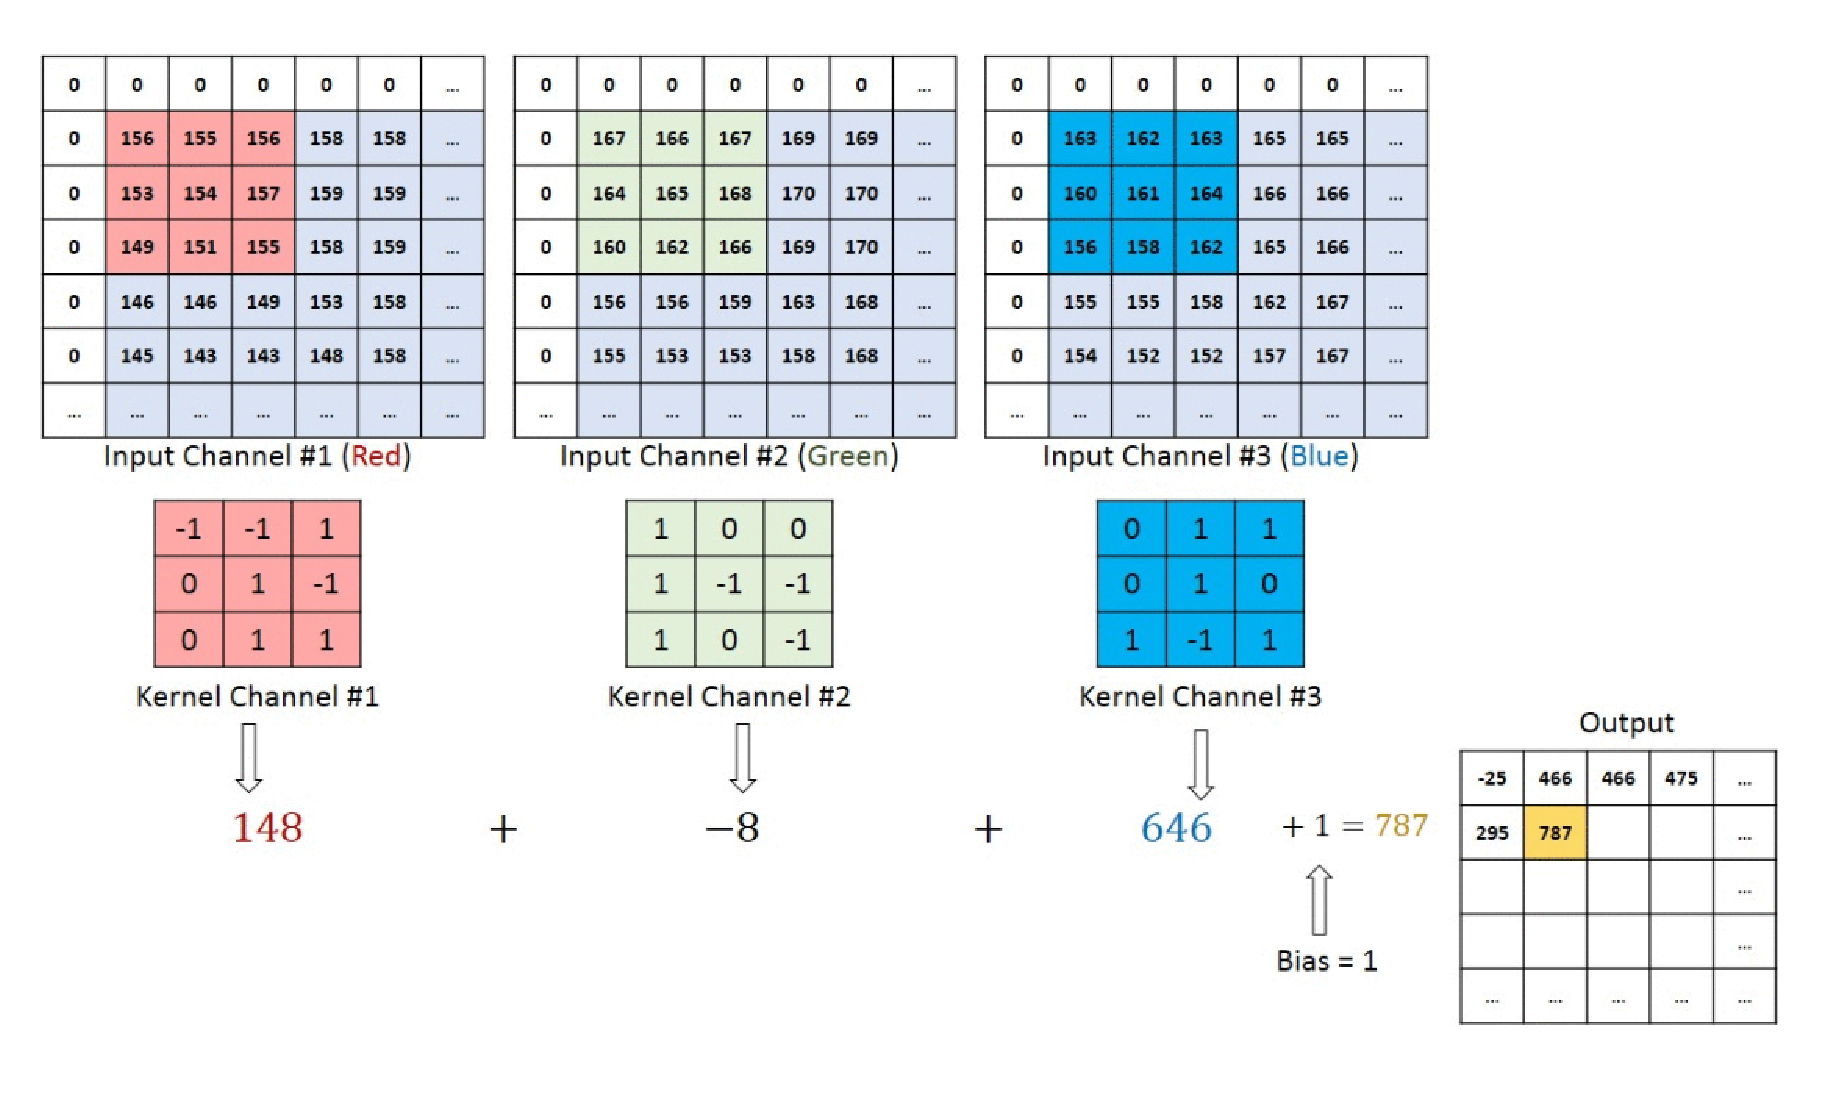
\includegraphics[scale=0.5]{finestra}
\caption{Ogni future map ha il suo kernel che scorre per tutta la dimensione dell'input.}
\end{figure}
\newpage
Un altro modo per regolare la dimensione delle feature map \`e tramite l'aggiunta di un bordo al volume di input, inserendo tutti valori nulli in proosimita del bordo. Con il parametro \textit{Padding} si denota lo spessore in pixel del bordo. L'uso di questo parametro ha il vantaggio di mantenere le dimensioni spaziali costanti dopo lo strato convoluzionale, migliorando le prestazioni. Questo perch\'{e} se gli strati non azzerassero gli input e realizzassero solo convoluzioni valide, allora la dimensione dei volumi si ridurrebbe di una piccola quantit\`{a} ad ogni convoluzione, in questo modo le informazioni ai bordi si perderebbero troppo rapidamente.\\
Sia $W_{out}$ la dimensione orizzontale (verticale) delle feature map di output e $W_{in}$ la corrispondente dimensione nell'input. Sia inoltre F la dimensione (orizzontale) del filtro e K il numero di filtri da utilizzare.\\
Vale la seguente relazione:
\begin{equation}
W_{out}=\frac{W_{in} -F+2\cdot Padding}{Stride}+1
\end{equation}
e la profondit\`{a} dell'output sar\`{a} pari a K.

\subsubsection{Strati di pooling}
Lo scopo degli strati di pooling \`e quello di unire caratteristiche simili (in quanto vicine) in una sola, per ridurre progressivamente la dimensione spaziale della rappresentazione. Di conseguenza si riduce anche la quantit\`{a} di parametri, che potebbero comportare un sovradattamento della rete.\\
Ogni strato appartenente alla profondit\`{a} dell'input viene suddiviso in piccoli quadrati, chiamati \textit{subsambling}, di dimensione  $r \times r$, con $r\in \mathbb{N}$ e  per ogni quadrato viene calcolato indipendentemente o il valore massimo (Max) o  la media (Avg) dei suoi neuroni.\\
Max e Avg sono gli operatori di aggregazione maggiormente utilizzati e sono invarianti per piccole tralslazioni. Riassumendo: una funzione di raggruppamento sostituisce l'output della rete in una determinata posizione con una statistica riassuntiva delle uscite vicine.\\
L'invarianza per traslazione \`e molto utile in quanto se una caratteristica \`e interessante in una parte dell'immagine, presumibilmnete lo sar\`{a} anche se \`e posizionata in un altro spazio.\\
Ad esempio, quando si determina se un'immagine contiene un volto, non \`e necessario conoscere la posizione degli occhi con "precisione pixel" perfetta, ma soltanto riscontrare la presenza di un occhio sul lato sinistro del viso e uno sul lato destro.\\
In altri contesti, \`e pi\'{u} importante conservare la posizione di una funzione. Ad esempio, se si vuole trovare un angolo definito da due spigoli che si incontrano con un orientamento specifico, bisogna verificare che sia preservata la posizione dei bordi in modo che essi si incontrino.\\
Passata in input un'immagine di volume $W_{in} \times H_{in} \times D$, lo strato di pooling di dimensione $F\times F$ e stride S produce un volume di dimensioni $W_{out} \times H_{out} \times D$, dove:
\begin{equation}
W_{out}=\frac{W_{in} - F}{S}+1
\end{equation}
Alternando ripetutamente queste due tipologie di strati, si arriva ad una configurazione spaziale unita dell'immagine di piccole dimensioni. In quest'ultima prospettiva  si passa a strati totalmente connessi, specialmente nell'ultimo strato dove l'output deve necessariamente essere una delle possibili classi.
\begin{figure}[!h]
\centering
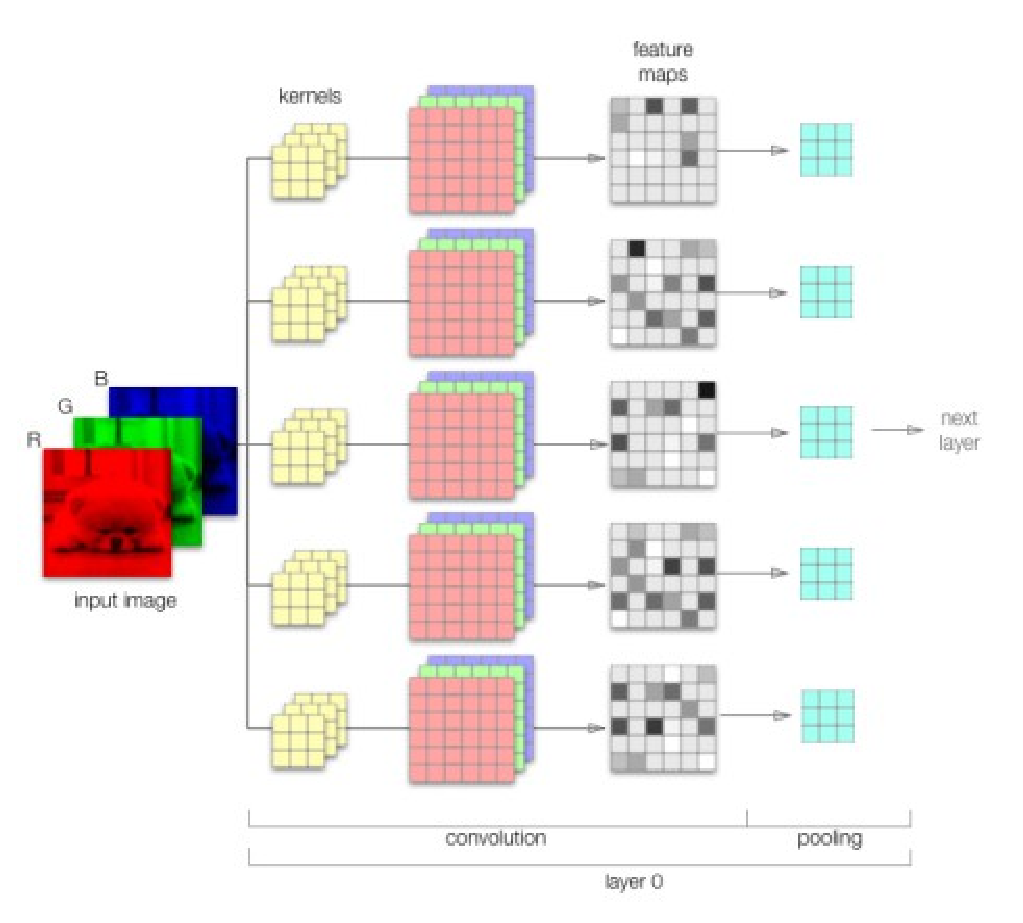
\includegraphics{panoramicaConv}
\caption{Struttura generale di una rete neurale convoluzionale}
\end{figure}




\chapter{Shazarch}
L'obiettivo di questa tesi, come detto pi\`{u} volte, \`{e} di trovare l'architettura ottimale per un modello di Deep Learning capace di riconoscere, quindi classificare, immagini di resti e monumenti presenti nell'area archeologica del Foro Romano a Roma. Vista la difficolt\`{a}, anche per un occhio umano, di riconoscere alcuni reperti si \`e pensato di inserire anche le informazioni relative alla geolocalizzazione di questi ultimi.\\
Questo modello \`e finalizzato per creare un'applicazione Android, chimata Shazarch, in grado di permettere al turista in visita al Foro Romano, di inquadrare l'oggetto di interesse e sapere cosa sta visualizzando in quel momento. Per fare questo si necessita di un modello di classificazione di deep learning, addestrato con un dataset di immagini provenienti dal sito archeologico e delle coordinate geografiche dei singoli monumenti. Si sta parlando di un algoritmo di apprendimento supervisionato, quindi il dataset che si utilizza deve contenere delle variabili rappresentanti le caratteristiche dell'oggetto da riconsocere, tra cui naturalmente anche un'etichetta. L'etichetta corrisponde alla classe di appartenenza dell'oggetto che, nel nostro caso, corrisponde ad un numero $n\in \{0,\cdots,29\}$, in quanto i reperti che la rete \`e in grado di riconoscere sono 30 ed in particolare sono:
\vspace{1cm}
\begin{center}
\begin{tabular}{lcl}
Arco di Settimio Severo & & Arco di Tito\\
Arco Partico & & Basilica Emilia \\
Basilica Julia & & Basilica Ulpia\\
Casa delle Vestali & & Colonna di Foca\\
Colonna Traiana & & Curia Julia \\
Domus Augustana & & Domus Flavia\\
Domus Tiberiana & & Foro di Cesare\\
Mercati di Traiano & & Portico degli Dei Consenti\\
Regia & & Tabularium\\
Tempio dei Castori & & Tempio Del Divo Giulio\\
Tempio della Concordia & & Tempio di Antonino e Faustina\\
Tempio di Saturno & & Tempio di Venere e Roma\\
Tempio di Vespasiano e Tito & & Tempio di Vesta\\
Tempio di Marte Ultore & & Umbilicus Urbis\\
Via Nova & & Volcanal
\end{tabular}
\end{center}
\vspace{1.5cm}
Per quanto riguarda le altre variabili si sono considerati i valori dei pixel delle immagini in formato RGB e di dimensione $3024\times 4032$. Inizialmente si era pensato di inserire anche le coordinate geografiche all'interno delle informazioni dell'immagine, ma questo avrebbe portato ad un fenomeno di underfitting, se non fossero state inserite delle distanze di riferimento all'interno delle informazioni dell'immagine, in quanto la rete non sarebbe stata in grado di trovare una funzione che generalizzi queste distanze (intese come distanze euclidee); viceversa se queste informazioni fossero state inserire si sarebbe andati incontro ad un sovraddatamento della rete: inserendo nuove coordinate di riferimento, la rete non le avrebbe riconsociute "vicine" a quelle del datset. Si \`e deciso quindi di non inserirle direttamente tra le informazioni delle immagini. Successivamente verr\`e{a} spiegato come sono state introdtte, non prima di aver finito di descrivere come \`e stato creato il dataset.\\
Il dataset di immagini deve essere abbastanza grande per far si che l'algoritmo abbia abbastanza immagini su cui addestrarsi e anche per verificare la sua accuratezza, si ricorda infatti che l'insieme di addestramento e di test(e/o di validazione) formano una partizione dell'insieme totale di partenza.\\
Il dataset utilizzato \`e composto da circa 40000 immagini, di cui una piccola parte originali, ovvero scattate fisicamente sul posto, le restanti sono state generate artificialmente tramite la libreria Augmentor. Questa libreria \`e progettata per aiutare l'incremento e la generazione artificiale di dati di immagine per attivit\`{a} di machine learning, tramite rotazioni, zoom, distorsioni ecc... Si \`e partiti da una media di 6 foto per classe e per ognuna di queste Augmentor ha generato 180 foto. Successivamente l'insieme di dati \`e stato diviso in modo che l'$80\%$ andasse a costituire l'insieme di addestramento e il $20\%$ quello di validazione. Come architettura per il modello si \`e optato per l'architettura pre-esistente mobileNet, descritta nel dettaglio nella sezione \ref{sez:mobileNet}, addestrata tramite il meotodo di discesa del gradiente (SGD) settato con il parametro di learning rate=0.1, dove nella fase di back propagation (\ref{back-prop})  batch size=100.
Una volta addestrata la rete, tensorflow salva il modello all'interno di un file, successivamente convertito con estensione ".lite". Questa conversione trasforma il modello in uno di tipo TensorFlow Lite, un formato che permette di 
utilizzare Android Studio: un ambiente di sviluppo integrato (IDE) per lo sviluppo per la piattaforma Android. All'interno del codice Java, linguaggio con cui si programma un'applicazione Android, sono state inserite le coordinate di geolocalizzazione.\\
Innanzitutto per capire come correlare questa informazione con quella data dal modello, si sono studiati gli eventi da analizzare per capire se questi fossero indipendenti o meno. Dato lo spazio campionario $\Omega ={C_1,\cdots,C_{30}}$, dove $C_i$ rappresentano le classi corripsondenti ai 30 monumenti, l'evento $E={C_{\hat{y}}=C_y}$ dove la classe predetta coincide con la classe effettiva e l'evento $F={monumento nelle vicinanze}$. Questi due eventi sono indipendenti, se cos\`{\i} non fosse si avrebbe che: $P(E\cap F)=P(F|E)\ldotp P(E)$, ma l'evento per cui la predizione \`e giusta non da nessuna informazione sulla distanza tra lei e l'osservatore, allora: $P(F|E)=P(F)$  e $P(E\cap F)=P(F)\ldotp P(E)$, che avviene se i due eventi sono indipendenti.\\
Sono stati implementati due metodi per considerare le posizioni GPS del visitatore. Una ,chiamata "GPS", considera la distanza tra il dispositivo ed il monumento osservato. Si \`e considerato che la probabilit\`{a} di un evento F, si comporta come una variabile aleatoria uniforme sull'intervallo (0,r), oltre il quale \`e plausibile pensare che il visitatore non possa vedere. Quindi:
\begin{equation}
P(X=d_i)=\begin{cases} 1 & \mbox{se }d_i\leq r \\ 0 & \mbox{altrimenti}\end{cases}
\end{equation}
dove $d_i$ \`e la distanza tra le coordinate dell'osservatore e il monumento di classe $C_i$.\\
L'altra applicazione sviluppata, chiamata "GPS Alarm", invece considera una circonferenza di raggio 20metri, centrata in un monumento che ne delimita la sua area "protetta". Se il visitatore non si trova all'interno di quest'area la probabilit\`{a} di osservare il monumento corrispondente ad essa \`e pari a zero, altrimenti \`e 1. Questo solo per poter conisderare solo i reperti che \`e ragionevole pensare un turista possa voler inquadrare. Naturalmente questi approcci non permettono di classificare un monumento da una distanza maggiore di quella considerata, anzi produrr\`{a} una classificazione errata, in quanto verranno considerate solo i monumenti in cui le coordinate del visitatore si trovano all'interno delle loro aree protette.\\
Ora che sono note la struttura e la logica con cui \` stata progettata Shazarch, si possono approfondire alcuni aspetti accennati in questa fase. 

\section{MobileNet}\label{sez:mobileNet}
MobileNet \`e un'architettura rilasciata da Google e resa disponibile open source, contenente una famiglia di modelli di computer vision per dispositivi mobili per TensorFlow. \`E stata progettata per massimizzare efficacemente l'accuratezza, tenendo presente le risorse limitate per un'applicazione integrata su dispositivo. Per questo motivo \`e stata scelta per adattarsi alla nostra esigenza di classificare immagini tramite un'applicazione installata su un dispositivo mobile. La particolarit\`{a} di questa architettura \`e l'uso di convoluzioni separabili per costruire reti neurali profonde leggere. L'intuizione di questi sviluppatori \`e stata di introdurre due semplici iperparametri che riescono ad equilibrare efficacemente latenza e accuratezza, permettendo all'architettura di adattarsi a diverse applicazioni. La latenza ,in informatica, di un sistema \`e l'intervallo di tempo che intercorre fra il momento in cui arriva l'input e il momento in cui \`e disponibile il suo output.\\
In altre parole: la latenza non \`e altro che una misura della velocit\`{a} di risposta di un sistema.\\
Ma che cosa si intende per convoluzioni separabili? Sono delle convoluzioni formate da due convoluzioni: una convoluzione in profondit\`{a} \`e una convoluzione con un filtro di dimensione $1\times 1$ chiamata convoluzione puntuale.
La convoluzione in profondit\`{a} applica un singolo filtro a ciascun canale di ingresso e all'output generato viene applicato il filtro della convoluzione puntuale. Riassumendo: la convoluzione standard consente di filtrare e combinare gli input in un nuovo set di output in un unico passaggio, mentre la convoluzione separabile lo fa in due passaggi, ognuno svolto da uno strato di convoluzione diverso.
\begin{figure}[h!]
\centering
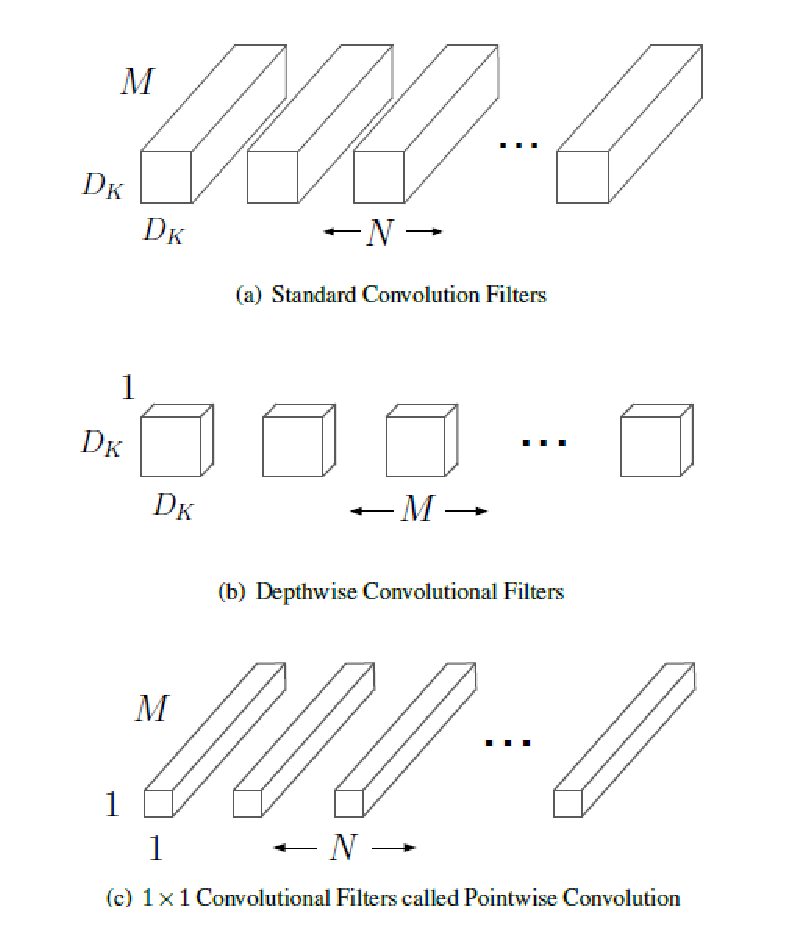
\includegraphics[scale=0.8]{fattorizzazione}
\caption{Fattorizzazione di una convoluzione standard in una convoluzione in profondit \`{a} e una convoluzione puntale.}
\end{figure}
\newpage
Questa fattorizzazione ha l'effetto di ridurre drasticamente il calcolo e la dimensione del modello. Infatti uno strato convoluzionale standard prende in input una feature map F di dimensioni: $D_F \times D_F \times M$ e produce in output la future map G di dimensioni: $D_G \times D_G \times N$, in seguito allll'applicazione di un filtro K di dimensioni: $D_K \times D_K \times M \times N$. Questo ha un costo computazionale pari a:
$$D_K \cdot D_K \cdot M \cdot N \cdot D_F \cdot D_F$$
Mentre nella convoluzione separabile si ha la convoluzione in profondit\`{a} che applica un filtro K' di dimensioni: $D_K\times D_K \times M$ ed ha un costo computazionale di:
$$D_K \cdot D_K \cdot M \cdot D_F \cdot D_F$$
Ora questi filtri devono essere combinati per creare nuove funzionalit\`{a}. Pertanto, per generare queste nuove caratteristiche, \`e necessario che lo strato con la convoluzione puntuale, faccia una combinazione lineare dell'uscita della convoluzione in profondit\`{a}, mediante la convoluzione con filtro di dimensione $1 \times 1$, di profondit\`{a} M e applicato agli N canali di output.\\
 Il suo costo \`e pari a:
$$M\cdot N \cdot D_F \cdot D_F$$
Quindi la convoluzione separabile ha un costo computazionale totale pari alla somma delle due convoluzioni:
$$ D_K\cdot D_k\cdot M\cdot D_F\cdot D_F + M\cdot N \cdot D_F \cdot D_F$$
Se si fa il rapporto dei costi computazionali dei due approcci, si ottiene una riduzione del calcolo di:
\begin{equation}
\frac{D_k\cdot D_k\cdot M\cdot D_F\cdot D_F + M\cdot N \cdot D_F \cdot D_F}{D_k\cdot D_k\cdot M\cdot N \cdot D_F \cdot D_F}=\frac{1}{N}+\frac{1}{D_K^2}
\end{equation}
L'architettura di MobileNet \`e quindi costituita da un primo strato con una convoluzione standard e da 12 convoluzioni separabili tutti implementati con una funzione di attivazione ReLu con batchnorm.\\
Abbiamo visto in precedenza (Cap. \ref{cap:reti}) l'importanza della funzione di attivazione all'interno dell'addestramento di una rete. Quando si calcola l'output di un singolo neurone si ha che il k-esimo nodo, in uno strato nascosto, ha il valore:
\begin{equation}
y_k=f_k(W_k \, x_{k-1})
\end{equation}
in questo caso h=ReLu. Se poniamo $z_k=W_k \, x_{k-1}$ , la batchnorm normalizza $z^k$, lo moltiplica per un parametro $a$ e gli aggiunge un altro parametro $b$ nel seguente modo:
$$\hat{z}_k=\frac{z_k-\mathbb{E}[z_k]}{\sqrt{V[z_k]}}\cdotp a +b$$
I parametri $\alpha$ e $\beta$ saranno anche loro minimizzati durante la ricerca dei pesi ottimali con la discecsa del gradiente (o altri metodi di minimizzazione).
Tornando all'architettura di mobileNet, dopo questi strati \`e presente un altro strato di convoluzione separabile, seguito da uno strato di Avg pooling (calcola la media dei suoi neuroni) che riduce la risoluzione spaziale ad 1 ed  infine lo strato di output fortemente connesso con funzione di attivazione Softmax per la classificazione.
Ricapitolando, come mostra la figura \ref{fig:mobileNet}, l'architettura ha:
\begin{itemize}
\item primo strato con convoluzione standard;
\item 26 strati nascosti con convoluzione separabile:
\item ultimo strato di output forteente connesso.
\end{itemize} 
per un totale di 28 strati, in quanto ogni strato nascosto \`e composto da una convoluzione separabile, che corrisponde a due strati consecutivi (convoluzione di profondit\`{a} e convoluzione puntuale).
\begin{figure}[!ht]
\centering
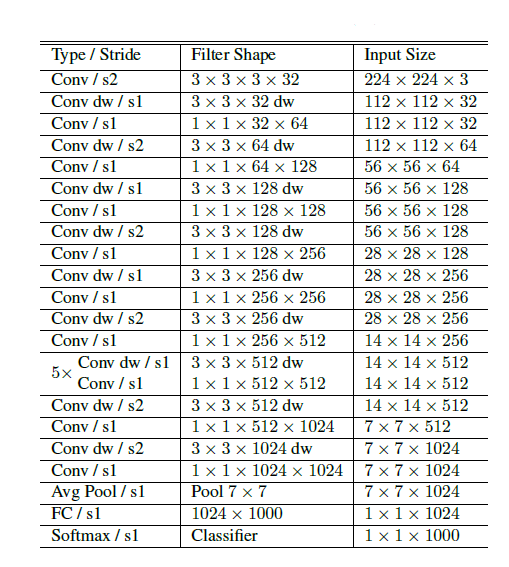
\includegraphics[scale=0.8]{mobileNet}
\caption{Struttura dell'architettura mobileNet.}
\label{fig:mobileNet}
\end{figure}


A partire da quaest'architettura si possono costruire modelli pi\`{u} piccoli e meno dispendiosi dal punto di vista computazionale, introducendo un "moltiplicatore di larghezza" $\alpha$ e un "moltiplicatore di risoluzione" $\rho$. 
Il ruolo del moltiplicatore di larghezza \`e quello di assottigliare uniformemente una rete su ciascun livello. Per un dato livello e moltiplicatore di larghezza $\alpha$, il numero dei canali di ingresso M diventa $\alpha \cdot M$ e il numero dei canali di uscita N diventa $\alpha \cdot N$. Quindi il costo computazionale di una convoluzione separabile di questo tipo \`e:
\begin{equation}
D_K\cdot D_K\cdot \alpha M\cdot D_F\cdot D_F + \alpha M\cdot \alpha N \cdot D_F \cdot D_F
\end{equation}
con $\alpha \in (0,1]$.\\
Il moltiplicatore di larghezza ha l'effetto di ridurre il costo computazionale e il numero di parametri in modo quadratico di circa $\alpha^2$.\\
Il Moltiplicatore di risoluzione $\rho$ serve a ridurre la dimensione dell'immagine. Viene infatti applicato all'immagine di input in modo che la rappresentazione interna di ogni livello viene successivamente ridotta dallo stesso moltiplicatore. Aggiungendo anche questo parametro il costo computazionale della rete con moltiplicatore di ampiezza $\alpha$ e moltiplicatore di risoluzione $\rho$ \`e:
\begin{equation}
D_K \cdot D_K  \cdot \alpha M\cdot \rho D_F\cdot \rho D_F + \alpha M\cdot \alpha N \cdot \rho D_F \cdot \rho D_F
\end{equation}
con $\rho \in (0,1]$ ed anche questo moltiplicatore ha l'effetto di ridurre il costo computazionale di $\rho^2$. \cite{mobileNet} \\
Per creare Shazarch \`{e} stata utilizzata l'architettura "standard" di mobileNet, ovvero dove gli iperparametri $\alpha$ e $\rho$ sono uguali a 1.\\
Inoltre si riocrda che la dimensione delle foto, con cui era stato costruito il dataset, era di $3024\times 4032$ pixels, mentre imageNet accetta solo immagini di dimensioni $224\times 224$, $192\times 192$, $160\times 160$ o $128\times 128$ pixels, quindi le immagini del dataset sono state ridimensionate in modo da soddisfare la dimensione richiesta. Questo ha comportato una perdita parziale di informazioni sulle immagini, ma era un prezzo da pagare per creare un'applicazione adattabile su un dispositivo mobile che non dispone di una memoria molto capiente.
\newpage



\section{TensorFlow}
TensorFlow (TF) \`{e} una libreria software open source, sviluppata da Google, utilizzata per implementare l'apprendimento automatico e i sistemi di deep learning. Essa fornisce API native in linguaggio: Python, C/C++, Java, Go, e RUST.\\
Per questo lavoro \`{e} stato utilizzato il linguaggio di programmazione Python.\\
In generale un algoritmo scritto in TF rispetta la seguente struttura:
\begin{enumerate}
\item Importare ed analizzare l'insieme di dati;
\item Creare colonne di caratteristiche per descrivere i dati;
\item Selezionare il tipo di modello;
\item Provare il modello;
\item Valutare l'efficacia del modello;
\item Lasciare che il modello addestrato faccia previsioni (test).
\end{enumerate}
Questa struttura \`{e} in linea con la descrizione di un generico algoritmo di apprendimento, descritto in (\ref{Costruzione}). La vera innovazione di TF risiede nella descrizione del modello, poich\'{e} lo fa costruendo un grafico computazionale: \textit{Data Flow Graph}. In questo grafico ogni nodo rappresenta l'istanza di un'operazione matematica, mentre ogni spigolo rappresenta un tensore, su cui vengono eseguite le operazioni.
\newpage
\begin{figure}[!ht]
\centering
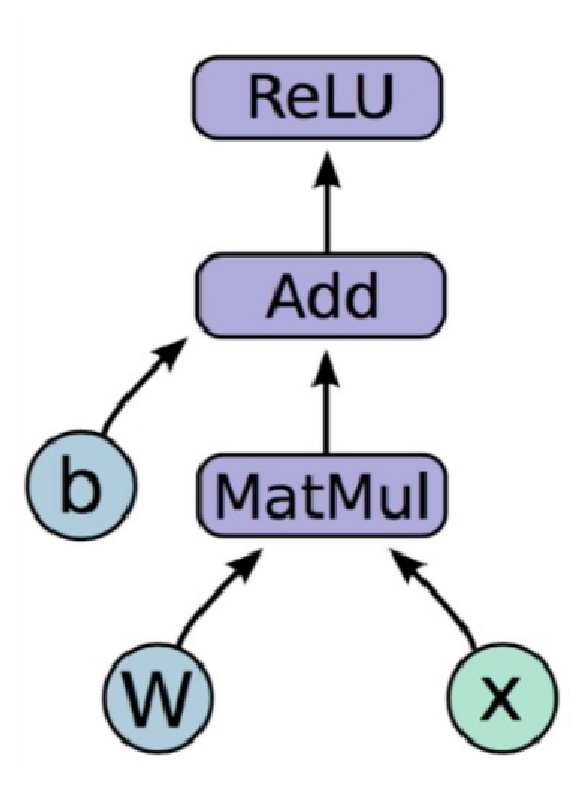
\includegraphics[scale=0.6]{flowgraph}
\caption{Data Flow Graph del calcolo di $ReLu(Wx+b)$.}
\end{figure}

\begin{defin}
Un \textbf{tensore} in TF \`{e} una matrice n-dimensionale di tipi di dati di base (es: float32, int32,string, ecc..). Viene chiamato tf.Tensor ed \`{e} descritto da tre parametri:
\begin{enumerate}
\item grado  (\textit{rank});
\item corpo (\textit{shape});
\item tipo (\textit{type}).
\end{enumerate}
\end{defin}
Il \textbf{grado} di un oggetto tf.Tensor \`{e} il suo numero di dimensioni.\\
Il \textbf{corpo} di un tf.Tensore \`{e} il numero di elementi in ogni dimensione. TF automaticamente deduce il corpo durante la costruzione del grafico.\\
Il \textbf{tipo} \`{e} il tipo di dato a cui appartongono gli elementi del tensore.\\
I principali tipi di tensori sono:
\begin{itemize}
\item Variabili (\textit{tf.Variable}): i parametri dell'algoritmo che verranno cambiati per ottimizzare l'algoritmo;
\item Costanti (\textit{tf.constant});
\item Segnaposto(\textit{tf.placeholder}): consentono di inserire dati e di creare operazioni per costruire il grafico computazionale, possono dipendere da altri dati ad esempio il risultato previsto di un calcolo. Possono essere usati pi\`{u} volte e non dare lo stesso risultato;
\item Tensore sparso (\textit{tf.SparseTensor}).
\end{itemize}
\begin{figure}[!h]
\centering
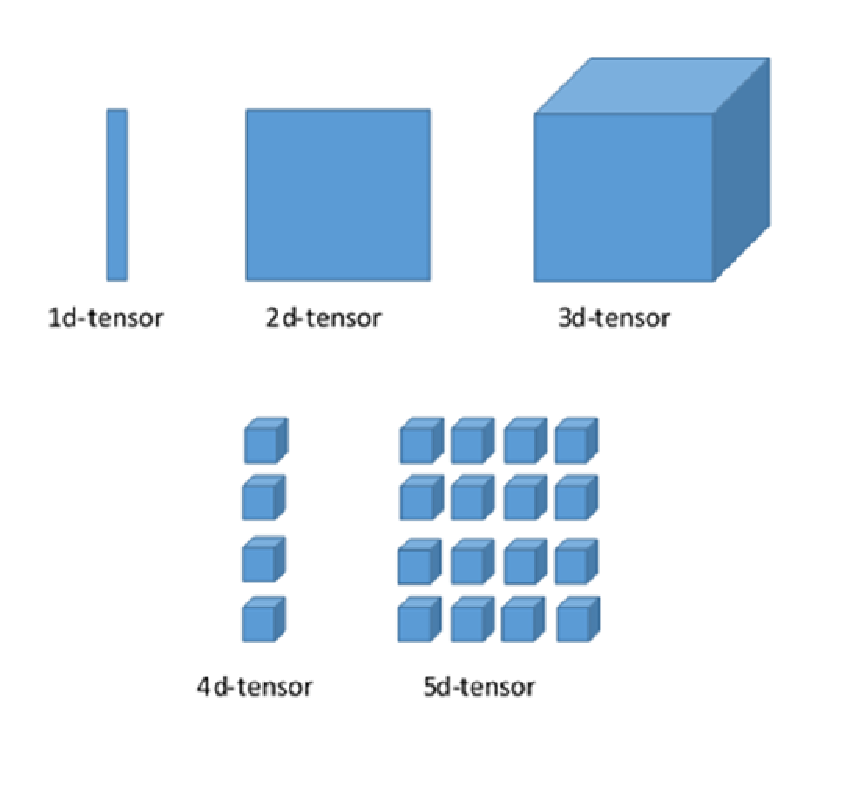
\includegraphics[scale=0.8]{tensori}
\caption{Strutture di tensori n-dimensionali, per alcune n.}
\end{figure}
\newpage
\subsection{Classificazione con KNN}
Di seguito viene riportato un esempio di codice per la classificazione di numeri scritti a mano estratti dal dataset di MNIST. L'algoritmo utilizzato \`{e} dei K-nearest neighbour,in due versioni: la prima non utilizza il batch size mentre la seconda si.
\begin{figure}[!h]
\centering
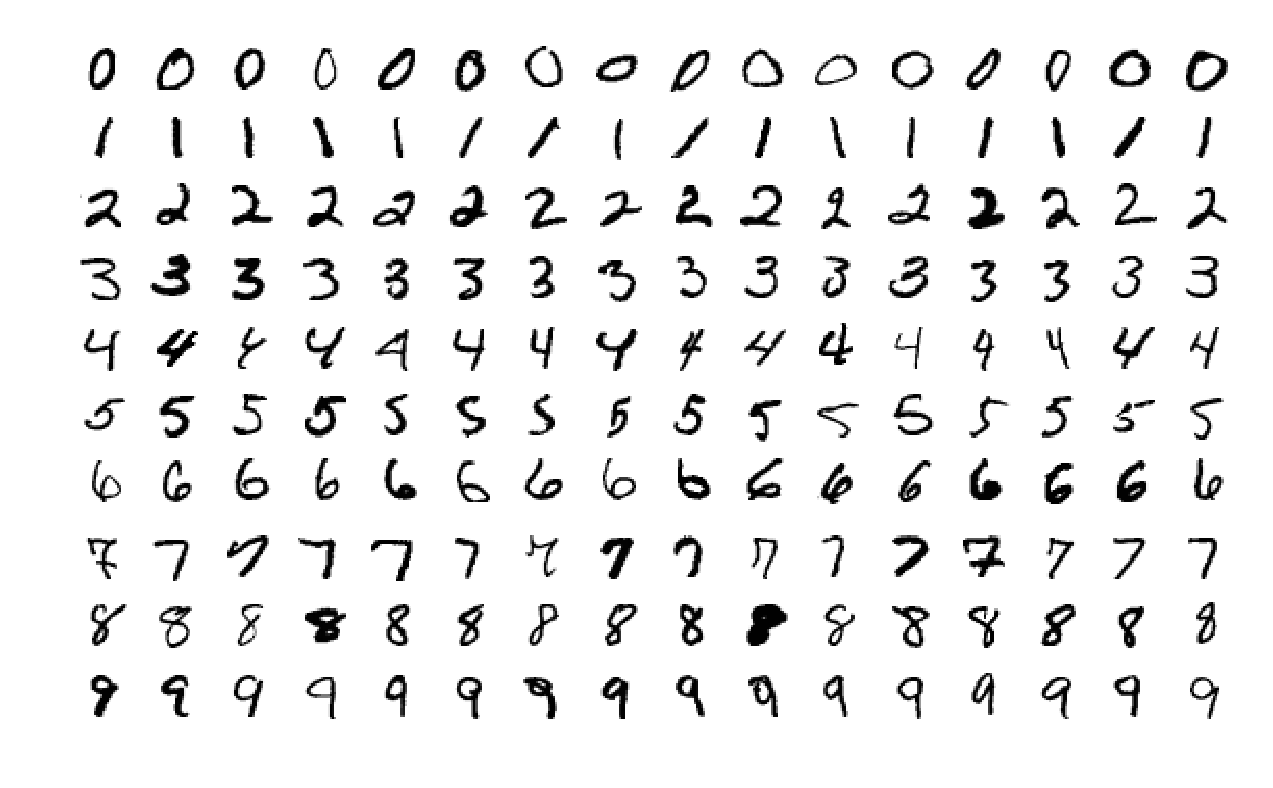
\includegraphics[scale=0.7]{MnistExamples}
\caption{Esempio di dati provenienti dal dataset Mnist}
\end{figure}


\textbf{Classificazione con k=5}
\begin{lstlisting}[language={Python},tabsize=2,basicstyle=\footnotesize]
import matplotlib.pyplot as plt
import numpy as np
import tensorflow as tf
from PIL import Image
from tensorflow.examples.tutorials.mnist import input_data
sess=tf.Session()
mnist=input_data.read_data_sets("MNIST_data/",one_hot=True)
train_size=2000
test_size=200
train_set=np.random.choice(len(mnist.train.images),train_size,
		replace=False)
test_set=np.random.choice(len(mnist.test.images),test_size,
		replace=False)
x_vals_train = mnist.train.images[train_set]
x_vals_test = mnist.test.images[test_set]
y_vals_train = mnist.train.labels[train_set]
y_vals_test = mnist.test.labels[test_set]
k = 5
x_data_train=tf.placeholder(shape=[None,784],dtype=tf.float32)
x_data_test=tf.placeholder(shape=[None,784],dtype=tf.float32)
y_target_train=tf.placeholder(shape=[None,10],dtype=tf.float32)
y_target_test = tf.placeholder(shape=[None, 10],dtype=tf.float32)
distance=tf.reduce_sum(tf.abs(tf.subtract(x_data_train,
			tf.expand_dims(x_data_test,1))),2)
neighbour_xvals,neighbour_indices=tf.nn.top_k(
			tf.negative(distance),k=k)
predict_indices=tf.gather(y_target_train, neighbour_indices)
count_of_predict=tf.reduce_sum(predict_indices,reduction_indices=1)
prediction=tf.argmax(count_of_predict,axis=1)
test_output=[]
ok=0
init=tf.global_variables_initializer()
sess.run(init)
for i in range(len(x_vals_test)):
    predictions=sess.run(prediction,feed_dict={x_data_train:
				x_vals_train,x_data_test:x_vals_test,y_target_train:
				y_vals_train, y_target_test: y_vals_test})
    test_output.extend(predictions)
    print("test n:",i, " Classe predetta:",test_output[i],
				"Classe vera:",np.argmax(y_vals_test[i]),"\n\r")
    if test_output[i]== np.argmax(y_vals_test[i]):
         ok=ok+1
accuracy = ok/len(x_vals_test)
print("Accuracy on test set:",accuracy)
\end{lstlisting}
Usando un insieme di addestramento di cardinalit\`{a} $2000$, e uno di test di cardinalit\`{a} $200$, si \`{e} ottenuta un'accuratezza dell'$89\%$ e il tempo impiegato di esecuzione \`{e} di $19.398$ secondi.\\
\textbf{Versione con batch size=10}
\begin{lstlisting}[language={Python},tabsize=2,basicstyle=\footnotesize]
import matplotlib.pyplot as plt
import numpy as np
import tensorflow as tf
from PIL import Image
from tensorflow.examples.tutorials.mnist import input_data
sess=tf.Session()
mnist=input_data.read_data_sets("MNIST_data/",one_hot=True)
train_size=2000
test_size=200
train_set=np.random.choice(len(mnist.train.images),
			 train_size,replace=False)
test_set=np.random.choice(len(mnist.test.images),
			test_size,replace=False)
x_vals_train=mnist.train.images[train_set]
x_vals_test=mnist.test.images[test_set]
y_vals_train=mnist.train.labels[train_set]
y_vals_test=mnist.test.labels[test_set]
k=5
x_data_train=tf.placeholder(shape=[None,784],dtype=tf.float32)
x_data_test=tf.placeholder(shape=[None,784],dtype=tf.float32)
y_target_train=tf.placeholder(shape=[None,10],dtype=tf.float32)
y_target_test=tf.placeholder(shape=[None,10],dtype=tf.float32)
distance=tf.reduce_sum(tf.abs(tf.subtract(x_data_train,
		tf.expand_dims(x_data_test,1))),2)
neighbour_xvals,neighbour_indices=tf.nn.top_k(
				tf.negative(distance),k=k) 
predict_indices=tf.gather(y_target_train,neighbour_indices)
count_of_predict=tf.reduce_sum(predict_indices,reduction_indices=1)
prediction=tf.argmax(count_of_predict,axis=1)
test_output=[]
actual_vals = []
batch_size=10
ok=0
init=tf.global_variables_initializer()
sess.run(init)
for i in range(int(np.ceil(len(x_vals_test)/batch_size))):
	min_index=i*batch_size
	max_index=min((i+1)*batch_size,len(x_vals_train))
	x_batch=x_vals_test[min_index:max_index]
	y_batch=y_vals_test[min_index:max_index]
	predictions=sess.run(prediction,feed_dict={x_data_train:
					x_vals_train,x_data_test:x_batch,
					y_target_train:y_vals_train,
					y_target_test: y_batch})
	test_output.extend(predictions)
	actual_vals.extend(np.argmax(y_batch, axis=1))
for i in range(len(x_vals_test)):
	print("test n:",i,"Classe predetta:",test_output[i],
				"Classe vera:", actual_vals[i],"\n\r")
	if test_output[i]==np.argmax(y_vals_test[i]):
		ok=ok+1
accuracy=ok/len(x_vals_test)
print("Accuracy on test set:",accuracy)
\end{lstlisting}
Utilizzando insiemi di addestramento e di test con le stesse cardinalit\`{a} dell'implementazione precedente, ma inserendo il parametro di batch size, si ottiene una velocit\`{a} di esecuzione maggiore: $15,535$ secondi ($\sim 4$s in meno). In accordo con la spiegazione dell'algoritmo in \ref{knn}, ci si aspettava un risultato di questo tipo. Purtroppo guadagnando velocit\`{a} di esecuzione si \`{e} perso qualcosa nell'accuratezza: da $89\%$ a $87\%$. Vale la pena sottolineare che, come detto pi\`{u} volte, non esiste un algoritmo migliore di un altro, ma il pi\`{u} adatto in base al problema da affrontare. Infatti se si aumenta il numero di esempi per l'insieme di addestramento e si inserisce il parametro di batch size, l'algoritmo sale di accuratezza pur mantenendo una velocit\`{a} di esecuzione bassa.  

\begin{figure}[h!]
\centering
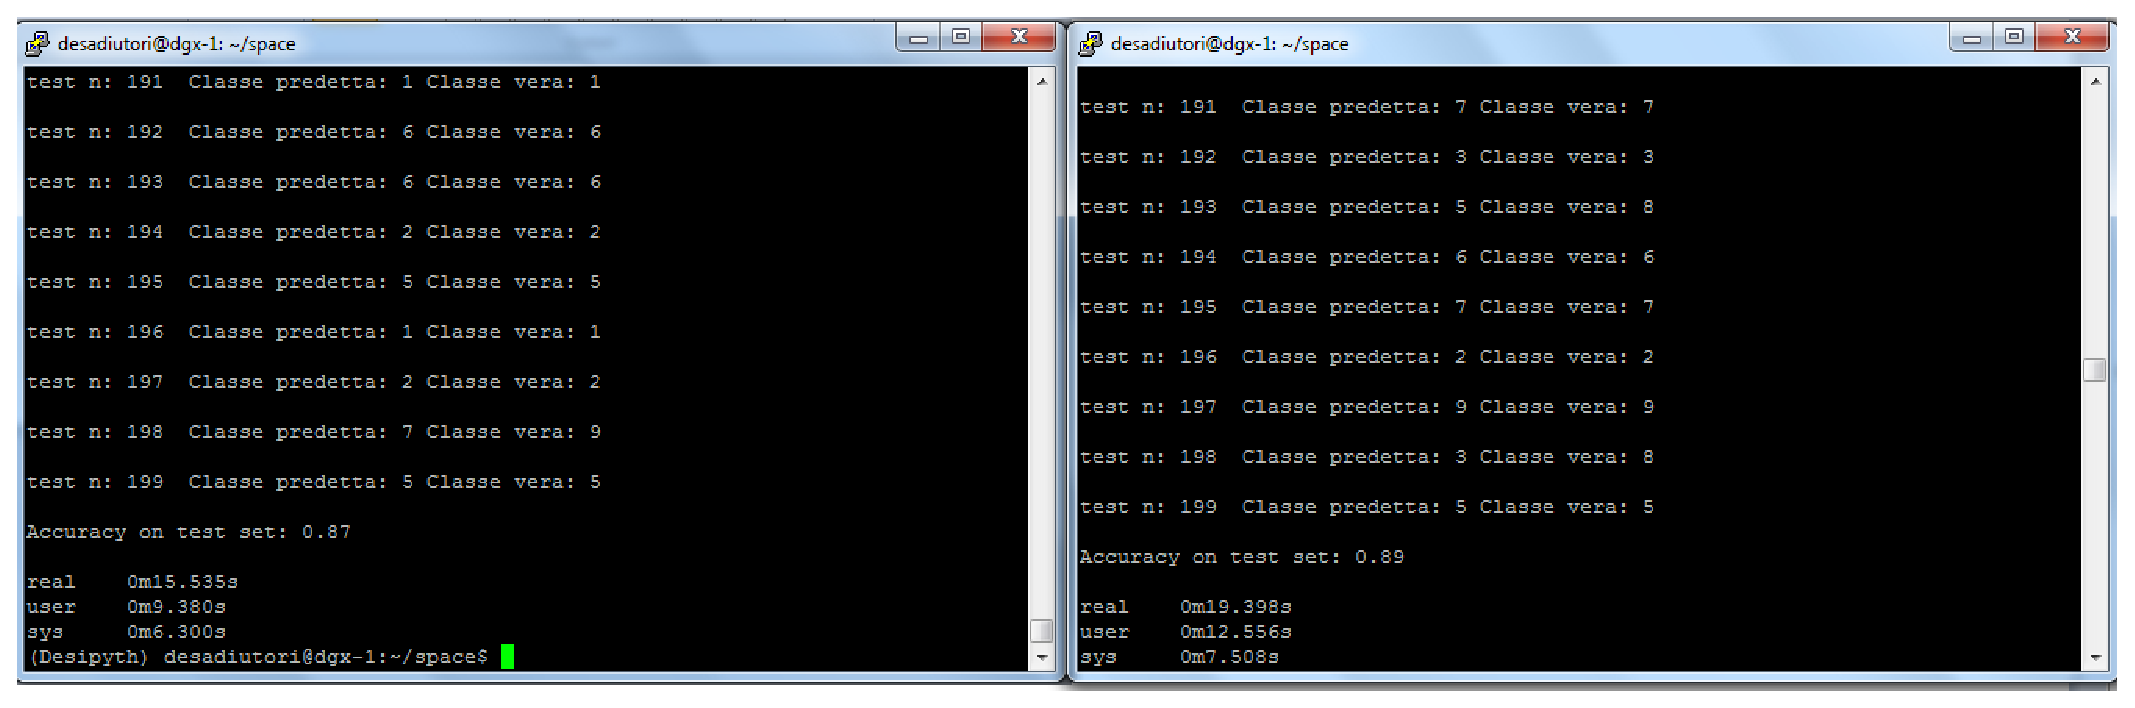
\includegraphics[scale=0.45]{schermata}
\caption{Schermate catturate dovo aver fatto il test: a sinistra test dell'algoritmo KNN con batch size, a destra senza.}
\end{figure}
\newpage

\subsection{Shazarch}
Di seguito si riporta il codice utilizzato per creare il modello per l'applicazione Shazarch.\\
Per prima cosa si \`e ampliato il dataset di partenza, tramite la generazione di foto artificiali con Augmentor con la seguente procedura generale: \cite{Augmentor}
\begin{enumerate}
\item Si istanzia un oggetto \textit{Pipeline};
\item Si definisce un numero di operazioni da eseguire;
\item Si eseguono le operazioni sull'oggetto Pipeline.
\end{enumerate}
\textbf{Passaggio 1- Creare un nuovo Pipeline:}\\
Per iniziare qualsiasi attivit\`{a} di incremento, \`e necessario innanzitutto inizializzare un oggetto Pipeline, che punta a una cartella (\textit{directory})  in cui \`e archiviato il set di dati dell'immagine originale:
\begin{lstlisting}[language={Python},tabsize=2,basicstyle=\footnotesize]
import Augmentor
p=Augmentor.Pipeline("/percorso/dove/risiedono/le/immagini")
\end{lstlisting}
La variabile p ora contiene un oggetto di tipo Pipeline ed \`e stata inizializzata con l'elenco di immagini trovate nella cartella di origine.\\
\textbf{Passaggio 2- Aggiungere operazioni a Pipeline:}\\
Una volta creato il Pipeline p, si possono aggiungere le operazioni da eseguire su di esso. Ad esempio, se si vuole creare un'immagine ruotata:
\begin{lstlisting}[language={Python},tabsize=2,basicstyle=\footnotesize]
p.rotate(probability=0.7, max_left_rotation=10, max_right_rotation=10)
\end{lstlisting}
In questo caso con una probabilit\`{a} del $70\%$, la foto sar\`{a} creata tramite una rotazione dell'originale verso sinistra o verso destra, entrambe di massimo $10\,�$, ovvero l'immagine verr\`{a} ruotata tra $-10$ e $10$ gradi.
\newpage
\begin{figure}[ht]
\centering
\includegraphics[width=55mm]{originale.eps}
\qquad\qquad
\includegraphics[width=55mm]{ruotata.eps}
\caption{Esempio di foto dell'Arco di Settimio Severo ruotata a destra.}
\end{figure}

Esistono molte altre operazioni che si possono applicare alle immagini, come ad esempio: zoom, conversione in bianco e nero, ritaglio, distorsione, riflessione ecc... 
 

\textbf{Passaggio 2- Eseguire le operazioni:}\\
Dopo aver aggiunto le operazioni necessarie, \`e possibile generare i nuovi dati modificati, utilizzando la funzione sample() e specificare il numero di immagini che si vuole ottenere, in questo caso $10.000$:
\begin{lstlisting}[language={Python},tabsize=2,basicstyle=\footnotesize]
p.sample(10000)
\end{lstlisting}
Dalla finestra del terminale apparir\`{a} una barra di avanzamento del processo durante la generazione dei campioni. Per impostazione predefinita, le immagini generate verranno salvate in una cartella denominata output, all'interno di quella contenente le immagini iniziali.\\
Infine Augmentor permette di eseguire un controllo per in dividuare eventuali doppioni generati e li cancella.\\
Una volta creato il dataset, si crea l'elenco delle etichette, che in questo caso corrisppondevano al nome delle cartelle che contenevano le immagini:\\
\begin{lstlisting}[language={Python},tabsize=2,basicstyle=\footnotesize]
_files = glob.glob('/percosdo/della/cartella/dataset/*')
labels = []
for f in _files:
    labels.append(f.split('/')[-1])
print(labels)
with open('/percordo/dove/salvare/file/label.txt',"a+") as f:
    for each in labels:
        f.write(each+'\n')
    f.close() 
\end{lstlisting}
Si crea un dizionario che associa un numero ad una classe:
\begin{lstlisting}[language={Python},tabsize=2,basicstyle=\footnotesize]
class_to_ix = {}
ix_to_class = {}
classes = [l.strip() for l in labels]
class_to_ix = dict(zip(classes,range(len(classes))))
ix_to_class = dict(zip(range(len(classes)),classes))
class_to_ix = {v:k for k,v in ix_to_class.items()}
\end{lstlisting}
Come detto in precedenza, poich\'e le immagini possedute avevano dimensioni maggiori da quelle compatibili con mobilNet, \`e stato necessario ridimensionarle:
\begin{lstlisting}[language={Python},tabsize=2,basicstyle=\footnotesize]
def load_images(path):
    all_imgs = []
    all_classes = []
    for i, subdir in enumerate(listdir(path)):
        imgs = listdir(join(path,subdir))
        class_ix = class_to_ix[subdir]
        print("{} - {} - {}".format(i,class_ix,subdir))
        for img_name in imgs:
            img_rr = mping.imread(join(path,subdir,img_name))
            if img_rr.shape==(224,224,3):
                all_imgs.append(img_rr)
                all_classes.append(class_ix)
            else:
                print("ERROR")
    print("All images : {}".format(len(all_imgs)))
    return np.array(all_imgs),np.array(all_classes)
\end{lstlisting}
Si \`e creato il modello mobileNet:
\begin{lstlisting}[language={Python},tabsize=2,basicstyle=\footnotesize]
base_model=MobileNet(input_shape=(224,224,3),include_top=False,
			input_tensor=Input(shape=(224,224,3)),pooling=None)

\end{lstlisting}
dove:
\begin{list}{-}{}
\item input\_shape \`e il formato delle immagini passate in input alla rete;
\item include\_top specifica se  includere lo strato completamente connesso nella parte iniziale della rete;
\item input\_tensor \`e la dimensione dell'input dell'immagine del modello;
\item pooling specifica se applicare il pooling finale, si pu\`{o} settare solo se include\_top=False.
\end{list}
Per questa configurazione sono stati settati $\alpha ,\rho =1$, che rappresentano rispettivamente il moltiplicatore di larghezza e di risoluzione. Non compaiono tra gli argomenti perch\`e, se omessi, sono settati gi\`{a} ad 1 di default. Discorso analogo per il valore relativo al dropout, che  di default vale $0.001$.\\
Si definscono le ultime operazioni da applicare all'output della rete, questo passaggio pu\`{o} essere inteso come un ultimo strato che, va a completare l'architettura .
\begin{lstlisting}[language={Python},tabsize=2,basicstyle=\footnotesize]
out = base_model.output
out = GlobalAvgPool2D(name='avg_pools26')(out)
out = Dropout(0.4)(out)
y_pred=Dense(n_classes,activation='softmax',kernel_initializer='random_uniform',
				kernel_regularizer=l2(.0005),name='last_layers26')(out)
\end{lstlisting}
\vspace{1cm}
Infine si crea il modello e lo si allena:
\begin{lstlisting}[language={Python},tabsize=2,basicstyle=\footnotesize]
model = Model(inputs=base_model.input,outputs=y_pred)
optimizer = SGD(lr=.01,momentum=.9)
model.compile(optimizer=optimizer,loss='categorical_crossentropy',
			metrics=['accuracy'])
model.fit(X_train,Y_train_cat,batch_size=100,epochs=10000,verbose=2,
			callbacks=[lr_sheduler,csv_logger,checkpointer],
					validation_data=(X_val,Y_val_cat),shuffle=True)
\end{lstlisting}
\vspace{1cm}
Con il metodo fit() si allena il modello, inserendo tra gli argomenti tutti i parametri necessari per settarlo, anche il metodo di minimizzazione da usare durante la fase di back-propagation, in questo caso SGD.\\
Ricapitolando, di seguito viene riportato l'intero codice:
\begin{lstlisting}[language={Python},tabsize=2,basicstyle=\footnotesize]
from __future__ import print_function
import os
import matplotlib.image as mping
from os import listdir
from os.path import join
import numpy as np
import glob
import tensorflow as tf
from keras.models import Model
from keras.applications.mobilenet import preprocess_input,decode_predictions
from keras.applications.mobilenet import MobileNet
from keras.layers import Dense, GlobalAvgPool2D, Input, Dropout
from keras.callbacks import ModelCheckpoint, CSVLogger
from keras.callbacks import ReduceLROnPlateau, LearningRateScheduler
from keras.optimizers import SGD
from keras.regularizers import l2
import keras.backend as K
from keras.utils.np_utils import to_categorical

_files = glob.glob('/percosdo/della/cartella/dataset/*')
labels = []
for f in _files:
    labels.append(f.split('/')[-1])
print(labels)
with open('/percordo/dove/salvare/file/label.txt',"a+") as f:
    for each in labels:
        f.write(each+'\n')
    f.close() 
assert(len(labels)==30)

train_path = '/percosdo/della/cartella/Train/'
valid_path = '/percosdo/della/cartella/Validation/'

class_to_ix = {}
ix_to_class = {}
classes = [l.strip() for l in labels]
class_to_ix = dict(zip(classes,range(len(classes))))
ix_to_class = dict(zip(range(len(classes)),classes))
class_to_ix = {v:k for k,v in ix_to_class.items()}

def load_images(path):
    all_imgs = []
    all_classes = []
    for i, subdir in enumerate(listdir(path)):
        imgs = listdir(join(path,subdir))
        class_ix = class_to_ix[subdir]
        print("{} - {} - {}".format(i,class_ix,subdir))
        for img_name in imgs:
            img_rr = mping.imread(join(path,subdir,img_name))
            if img_rr.shape==(224,224,3):
                all_imgs.append(img_rr)
                all_classes.append(class_ix)
            else:
                print("ERROR")
    print("All images : {}".format(len(all_imgs)))
    return np.array(all_imgs),np.array(all_classes)
    
X_train, Y_train = load_images(train_path)
X_val, Y_val = load_images(valid_path)

n_classes = len(labels)
n_classes
Y_train_cat = to_categorical(Y_train, n_classes)
Y_val_cat = to_categorical(Y_val, n_classes)

session = tf.Session()
K.set_session(session)
base_model=MobileNet(input_shape=(224,224,3),include_top=False,
				input_tensor=Input(shape=(224,224,3)),pooling=None)
out = base_model.output
out = GlobalAvgPool2D(name='avg_pools26')(out)
out = Dropout(0.4)(out)
y_pred=Dense(n_classes,activation='softmax',kernel_initializer='random_uniform',
				kernel_regularizer=l2(.0005),name='last_layers26')(out)
model = Model(inputs=base_model.input,outputs=y_pred)
optimizer = SGD(lr=.01,momentum=.9)
model.compile(optimizer=optimizer,loss='categorical_crossentropy',
			metrics=['accuracy'])
checkpointer=ModelCheckpoint(filepath='/percosdo/dove/salvare/file/model.
			{epoch:02d}-{val_loss:.2f}.hdf5', verbose=1, save_best_only=True)
csv_logger = CSVLogger('/percosdo/dove/salvare/file/model.log')
def schedule(epoch):
    if epoch < 15:
        return .01
    elif epoch < 28:
        return .002
    else:
        return .0004
    
lr_sheduler = LearningRateScheduler(schedule)
model.fit(X_train,Y_train_cat,batch_size=100,epochs=10000,verbose=2,
			callbacks=[lr_sheduler,csv_logger,checkpointer],
			validation_data=(X_val,Y_val_cat),shuffle=True)
\end{lstlisting}
Il modello appena creato \`e di tipo tensorflow, ma per poterlo esportare, in modo che possa essere sfruttato, ha bisogno di essere convertito. In questo caso si necessita di un formato di tipo tensorflowLite, che \`e compatibile con AndroidStudio: l'ambiente di sviluppo scelto per creare l'applicazione. Nel prossimo paragrafo verr\`{a} illustrato l'utilizzo di AndroidStudio.
\newpage
\section{AndroidStudio}
Android Studio \`e un ambiente di sviluppo integrato (IDE) per lo sviluppo per la piattaforma Android. Basato sul software IntelliJ IDEA, \`e stato progettato specificamente per lo sviluppo di applicazioni Android. \`{E} disponibile in download gratuito su Windows, Mac OS X e Linux, sostituisce gli Android Development Tools (ADT) di Eclipse, diventando l'IDE primario di Google per lo sviluppo nativo di applicazioni Android.\\
Alla base di ogni applicazione Android ci sono quattro tipi di componenti: Activity, Service, Content Provider e BroadcastReceiver. \\
Un'\textbf{Activity} \`e un'interfaccia utente. Ogni volta che si usa un'App, generalmente, si interagisce con una o pi\`{u} schermate, mediante le quali si consultano dati o si immettono input. Essa \`e il punto di partenza di ogni applicazione ed \`e la componente con cui l'utente ha il contatto pi\`{u} diretto.\\
Un \textbf{Service} svolge un lavoro, generalemente lungo e continuato, che viene svolto interamente in \textit{background} senza bisogno di interazione diretta con l'utente. I Service hanno un'importanza basilare nella programmazione proprio perch\'{e}, spesso, preparano i dati che le activity devono mostrare all'utente, permettendo una reattivit\`{a} maggiore nel momento della visualizzazione.\\
Un \textbf{Content Provider} nasce con lo scopo della condivisione di dati tra applicazioni, permettendo di condividere, nel sistema, contenuti custoditi in un database, su un file o reperibili mediante accessi in Rete.\\
Un \textbf{Broadcast Receiver} \`e un componente che reagisce ad un invio di messaggi a livello di sistema, con cui Android notifica l'avvenimento di un determinato evento, ad esempio l'arrivo di un SMS o di una chiamata. Questi componenti sono utili per la gestione istantanea di determinate circostanze speciali.\\
Un \textbf{Intent} \`e un oggetto che associa due componenti separate, come due attivit\`{a}, in seguito dell'invocazione di una per l'altra. Esso rappresenta infatti l'intento di fare qualcosa, senza che la componente chiamante cessi la sua esistenza.
Un \textbf{Fragment} \`e strettamente legato alla propria activity, dalla quale riceve eventi in input, che possono essere elaborati mentre l'attivit\`{a} \`e in esecuzione. La particolarit\`{a} di questo componente risiede nel fatto che, un Fragment pu\`{o} avere un'interfaccia utente totalmente sua, sempre per\`{o} all'interno di quella dell'activity. Si pu\`{o} pensare ad esso come un frammento dell'Activity, indipendente da essa, un esempio \`e dato da i menu a tendina al lato della schermata di un'applicazione.\\
All'interno di AndroidStudio il linguaggio utilizzato \`e quello Java, per le parti delle componenti principali. Mentre le parti che descrivono l' "estetica" dell'applicazione, ovvero i \textit{layout}, sono scritti in .xml.\\
Quando si inizia un progetto Android, la prima cosa da fare \`e istanziare l'activity principale, senza la quale non pu\`{o} essere costruita un'applicazione.\\
La mainActivty, dal punto di vista del codice,  \`e una classe che estende la super classe Activity e dalla quale eredita dei metodi che verranno implementati tramite \textit{override}. In generale ci\`{o} che collegher\`{a} i layer con la classe sar\`{a} il documento, in formato .xml, chiamato: AndoridManifest. Esso raccoglie le informazioni necessarie al sistema per far girare qualsiasi porzione di codice all'interno dell'applicazione. Tra le altre cose il Manifest si occupa delle seguenti cose:
\begin{itemize}
\item Da un nome al package Java dell'applicazione, che \`e anche un identificatore univoco della stessa;
\item Descrive le componenti dell'applicazione, nomina le classi e pubblica le loro "competenze";
\item Determina quali sono i processi che ospiteranno i componenti dell'applicazione;
\item Dichiara i permessi ai quali pu\`{o} accedere l'app, e i permessi necessari alle altre app per interagire con essa;
\item Dichiara il livello minimo di API Android che l'app richiede;
\item Elenca le librerie necessarie all'app per girare.
\end{itemize}
Per questi motivi, il Manifest pu\`{o} essere visto come il vero cuore di un'applicazione android.\\
\subsection{Shazarch}
L'applicazione creata si basa su 4 cartelle principali:
\begin{enumerate}
\item manifests;
\item java;
\item assets;
\item res.
\end{enumerate}
Nella cartella manifests risiede l'AndoridManifest.xml citato poco fa.\\
La cartella java racchiude tutte le classi e le interfacce utilizzate per creare le componenti. Nello specifico racchiude le classi:
\begin{list}{-}{}
\item AutoFitTextureView: ridimensiona la schermata alla dimensione del dispositivo ospitante;
\item CFragment: crea l'interfaccia con cui l'utente interagisce;
\item Classifier: importa il modello di classificazione tensorflowLite e ne rielabora l'output;
\item GPS: riceve le informazioni sulla geolocalizzazione e opera su di esse;
\item LogoView: fa visualizzare il risultato della classificazione;
\item MainActivity: lancia e gestisce le classi CFragment e GPS;
\item Splash: Crea la schermata di apertura dell'applicazione e lancia la MainActivity.
\end{list} 
Insieme alle classi risiedono anche le interfacce:
\begin{list}{-}{}
\item GPSActivity: necessaria per tutte quelle parti di codice che utilizzano un oggetto di tipo GPS;
\item ParentView: necessaria per la classe LogoView.
\end{list}
Nella cartella assets, si inseriscono tutti i file che l'applicazione deve caricare. Qui va inserito, ad esempio, il modello addestrato.\\
All'interno di res risiedono cartelle riguardanti l'impaginazione, lo stile ed il formato del testo, animazioni ecc...\\
Per capire quale fosse l'architettura ottimale, sono state realizzate 3 applicazioni:
\begin{itemize}
\item Archlite: senza coordinate di geolocalizzazione;
\item GPS: con coordinate di geolocalizzazione, considera la distanza tra monumento e osservatore; 
\item Alarm: con coordinate di geolocalizzazione, considera la presenza del visitatore intorno al monumento.
\end{itemize}
Introdcendo l'acceso al dispositivo GPS, bisogna inserire nell'AndoridManifest la richiesta ai permessi:
\begin{lstlisting}
<uses-permission android:name="android.permission.
			ACCESS_FINE_LOCATION"/>
<uses-feature android:name="android.hardware.location.gps"/>
\end{lstlisting}
altrimenti l'applicazione non potrebbe funzionare. La scelta della geolocalizzazione tramite dispositivo GPS  \`e dovuta dal fatto che entrambe le applicazioni devono funzionare senza una connessione dati attiva.


\section{Conclusioni}
Attraverso la piattorma NVIDIA DGX-1, fornita dal dipartimento di Roma3, \`e stato addestrato il modello di depp learning costruito. Le applicazioni Archlite e GPS sono state testate direttamente sul sito archeologico del Foro Romano. Durante il test sono state fatte all'incirca 400 rilevazioni per 13 siti su 30, una media di 30 foto a reperto, diversificate sia per angolatura che per distanza dal soggetto.\\
I risultati ottenuti hanno mostrato un'architettura non ancora ottimale: entrambi i modelli hanno un' accuratezza del $52\%$  e una diversificazione tra le due applicazioni da migliorare. Evidentemente la probabilit\`{a}, calcolata basandosi sulla distanza tra il monumento ed il dispositivo, va aumentata di qualche ordine di grandezza. La GPS provata si basa sulla distribuzione uniforme su un intervallo (0,d), dove d  \`e la distanza, che  \`e lineare.\\ 
In GPS, l'etichetta predetta ha una probabilit\`{a} maggiore di "match" con l'etichetta effettiva, in confronto ad Archlite, quando ci si trova in prossimit\`{a} del sito, come mostrato nella figura: \ref{fig:vicina}.
\begin{figure}[!ht]
\centering
\includegraphics[width=55mm]{archLite2}
\qquad\qquad
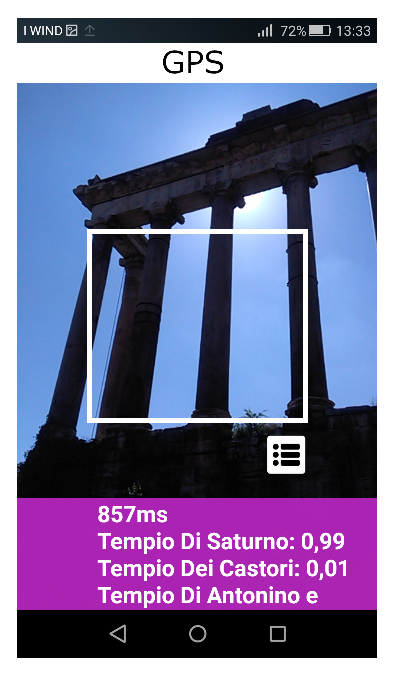
\includegraphics[width=55mm]{GPS2}
\caption{Schermata catturata ai piedi del Tempio di Saturno, a sinistra: il risultato dell'app ArchLite, a destra: il risultato dell'app GPS}
\label{fig:vicina}
\end{figure}

Viceversa la probabilit\`{a} \`e pi\`{u} bassa quando la foto risulta "panoramica", ovvero quando il sito di interesse \`e lontano dall'obiettivo della fotocamera. Si \`e osservato che nei casi in cui si  \`e vicini al sito, se la predizione \`e corretta, la probabilit\`{a} registrata \`e sempre molto alta, mentre quando la previsione \`e errata, l'app GPS registra una probabilit\`{a} pi\`{u} bassa, si veda la figura \ref{fig:panoramica}. Denotando un comportamento coerente con la "filosofia" con cui \`e stato costruito.

\newpage
\begin{figure}[!ht]
\centering
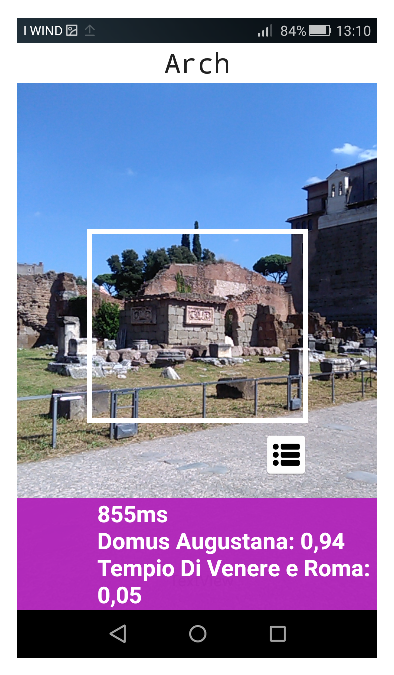
\includegraphics[width=55mm]{archLite}
\qquad\qquad
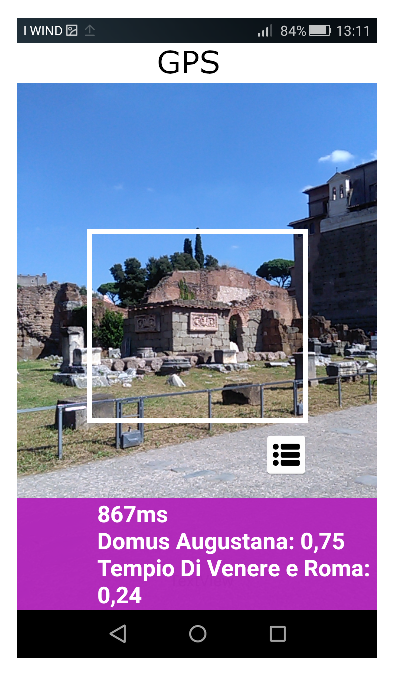
\includegraphics[width=55mm]{GPS}
\caption{Schermata catturata della Basilica Emilia, erroneamente classificata. A sinistra la predizione dell'app ArchLite, a destra l'app GPS.}
\label{fig:panoramica}
\end{figure}


Si \`e riscontrato un fenomeno di overfitting: l'etichetta corrispondente alla  "Domus Augustana" \`e spesso tra i risultati pi\`{u} probabili, se non il pi\`{u} probabile. Il fenomeno si \`e verificato in quanto, l'area della Domus Augustana \`molto vasta, perci\`{o} il numero di foto necessarie al riconoscimento sono pi\`{u} numerose. La rete quindi \`e stata allenata troppo con queste immagini e tende a riconoscere sopratutto loro. Proprio a causa di questo comportamento, i risultati sono stati inficiati dalla predominanza di questa etichetta. Nei casi in cui il valore predetto non corrisponde a quello effettivo, la Domus Augustana compare come risultato pi\`{u} probabile nel $50\%$ dei casi. Come nella figura (\ref{fig:panoramica}) dove, invece di classificare l'immagine come la Basilica Emilia, l'errore di predizione \`e ricaduto sulla Domus Augustana.\\
Quando il modello viene testato, tramite il suo insieme di validazione, su DGX l'accuratezza \`e molto elevata, misurando in alcuni casi anche il $100\%$ di accuratezza. Mentre durante il test ai Fori l'accuratezza \`e molto bassa: $53\%$ per entrambe le applicazioni ma, nell'analizzare i valori di probabilit\`{a} registrati, GPS sembra essere (seppur di poco) pi\`{u} attendibile, anche se lontana dall'essere ottimale, ma ci sono margini di miglioramento possibili.


\clearpage
\addcontentsline{toc}{chapter}{Bibliografia}
\nocite{*}
\bibliographystyle{unsrt}
\bibliography{bibliografia}

\end{document}
